\chapter{Energy Estimators}
\label{chap:MoreStuff}

\chapterquote{There, sir! that is the perfection of vessels!}
{Jules Verne, 1828--1905}

%========================================================================================
%========================================================================================

\section{Calibration}

%========================================================================================

\subsection{Calibration in the particle flow paradigm}
% Results use detector model 85 and calibration variant 71

\textcolor{red}{TODO: Trim down.}

In any experiment, calibration is essential for ensuring reliability in measured quantities and the linear collider will be no exception to this.  At the linear collider there will be several measured quantities each of which will be converted into a measure of the energy deposited in a given region of the detector.  These fall into two distinct classes (i) calorimeter energy deposits and (ii) track deposits.  The focus of this section will be on the energy deposits in the calorimeter and the procedure developed to ensure that they are reliable.  

Calorimeter energy deposits are an essential building blocks for the application of the particle flow paradigm.  The separation of energy deposits from charged and neutral particles in the calorimeters is crucial to achieve the full potential of particle flow and this is only possible with accurate energy estimators for those energy deposits.  A robust calibration scheme has been developed and will be discussed in the following chapter. 

The other crucial energy deposit used in particle flow calorimetry are track energy deposits.  These are also crucial to physics performance, however, in the particle flow paradigm these energy deposits are topologically related to the energy of the reconstructed particle.  A spatial helix fit is applied to the track energy deposits which when combined with knowledge of the magnetic filed yields the momentum of the particle producing the track.  Therefore, there is no direct relationship between the energy deposited by the monte-carlo particle in the active medium and the energy of the reconstructed energy.  Therefore, precise calibration of the energy deposited by a charged particle track is less crucial than for calorimeter energy deposits.  For this reason the focus of this chapter is on the calibration of calorimeter energy deposits. 

Calibration of the linear collider simulation extends beyond the raw calorimeter hits and into the particle flow algorithm itself.  The fine calorimeter granularity required for particle flow calorimetry yields excellent physical separation of hadronic and electromagnetic showers.  Thanks to sophisticated particle identification occurring within PandoraPFA it is possible to distinguish hadronic and electromagnetic showers, which allows for distinct treatments of the hadronic and electromagnetic energy estimators.  This distinction can be used to produce a response from the calorimeter that is compensating despite the intrinsic response being non-compensating.  A compensating calorimeter would give significant improvements to the energy resolution for the detector.

Two treatments designed to achieve a compensating response from the calorimeters are discussed.  The both involve rescaling the energies, the first rescaling is applied using a series of fixed energy independent constants, while the second uses the energy density of the calorimeter hits in the shower to determine the energy rescaling factor.

%========================================================================================

\subsection{Calibration and detector optimisation}
Optimising the detector at a future linear collider will be crucial to exploit the full physics potential available to it.  An extensive optimisation of the calorimeters was performed and the results can be found in chapter \ref{sec:optimisationstudies}.  For each detector model considered in this study the calibration procedure outlined in this section was applied to ensure optimal performance was achieved.  This made unbiased comparison between detector models performance possible and ensured reliability in the conclusions drawn from this study.

%========================================================================================

\subsection{Calibration Goals}
The calibration procedure aims to accurately set parameters related to four aspects of the reconstruction, which are:

\begin{enumerate}
\item \textbf{Digitisation of calorimeter hits}.  Digitisation in this sense is the estimation of the energy deposited within a calorimeter cell, the active and absorber layers, based on the signal measured in the sensitive region of the cell, the active layer.  
\item \textbf{Minimum ionising particle (MIP) scale setting in the digitisation processor and PandoraPFA}.  The MIP scale has to be set in the digitiser as it simulates the response of the readout technology including a maximum readout value, which is in units of MIPs.  The digitiser also applies a minimum active layer cell energy threshold, in units of MIPs, that has to be passed for creation of a calorimeter hit to occur.  This is designed to veto noise that would be present in a real detector.  PandoraPFA uses the MIP scale to place further threshold cuts on the cell energy that must be exceeded before a calorimeter cell is used in the reconstruction.  Both of these thresholds are designed to veto noise that would be present in a real detector.  While no noise is applied to the simulation these cuts are still applied to better represent the performance of a real detector. 
\item \textbf{Electromagnetic and hadronic scale setting in PandoraPFA}.  As discussed in chapter CALORIMETER CHAPTER, the response of a calorimeter to electromagnetic and hadronic showers is different due to the fundamentally different mechanisms governing their propagation.  One key difference between the two is the presence of an invisible energy component in the hadronic shower.  Therefore, the reported energy from a calorimeter to a hadronic showers will be lower than that of an electromagnetic shower.  To account for effects such as this and to account for energy losses due to the application of noise vetoing cuts in PandoraPFA the PFO energies are rescaled by PandoraPFA depending on whether the PFO has showered electromagnetically or hadronically.  Determination of these scaling factors is the setting of the electromagnetic and hadronic energy scales.  
\item \textbf{Retraining photon likelihood data}.  The PandoraPFA algorithm uses likelihood data to determine whether a reconstructed object is a photon.  This likelihood data has to be retrained for every new detector model considered. 
\end{enumerate}

Each of these aspects needs separately addressing for each new detector model considered.  The ordering of each of these calibration steps also had to be taken into consideration as it is possible to get interference between the different stages if applied in the wrong order.  

%========================================================================================

\subsection{Digitisation}
Calibration of the digitisation of the calorimeter hits involves accurately estimating the energy deposited in a calorimeter cell, in both the active and absorber layers, based on the energy deposited in the sensitive element of the calorimeter, the active layer.  The relationship between the energy deposited in the active layers and the absorber layers of a calorimeter is linear as the energy deposited in both layers are proportional to the number of charged tracks passing through them.  The ratio of the calorimeter cell energy to the energy deposited in the active layers is hereby called the digitisation constant.  
.
The digitisation constants depend upon several aspects of the detector including the material properties of the calorimeters, the magnetic field strength and energy losses occurring within the gaps between the active and absorber layers.  To account the effect of instrumented read out technology that would exist in a completed calorimeter some material is included in the simulation around the active and absorber layer.  In comparison to the absorber layer this extra material adds little to the detector, but energy losses here are accounted for in digitisation.  

%========================================================================================

\subsubsection{ECal Digitisation}
\label{sec:ecaldigi}
The procedure for determining the digitisation constants in the ECal involved the simulation of single $\gamma$ events at $E_{MC} = 10$ GeV.  $\gamma$ events are ideal for calibration of the ECal as in the particle flow paradigm $\gamma$ energy measurements are made primarily within the ECal.  Also at this energy $\gamma$s are largely contained within the ECal, as shown in figure \ref{fig:ecaldigiphotonsplit}, making them ideal for isolating the ECal digitisation calibration from that of the HCal digitisation calibration.   

\begin{figure}
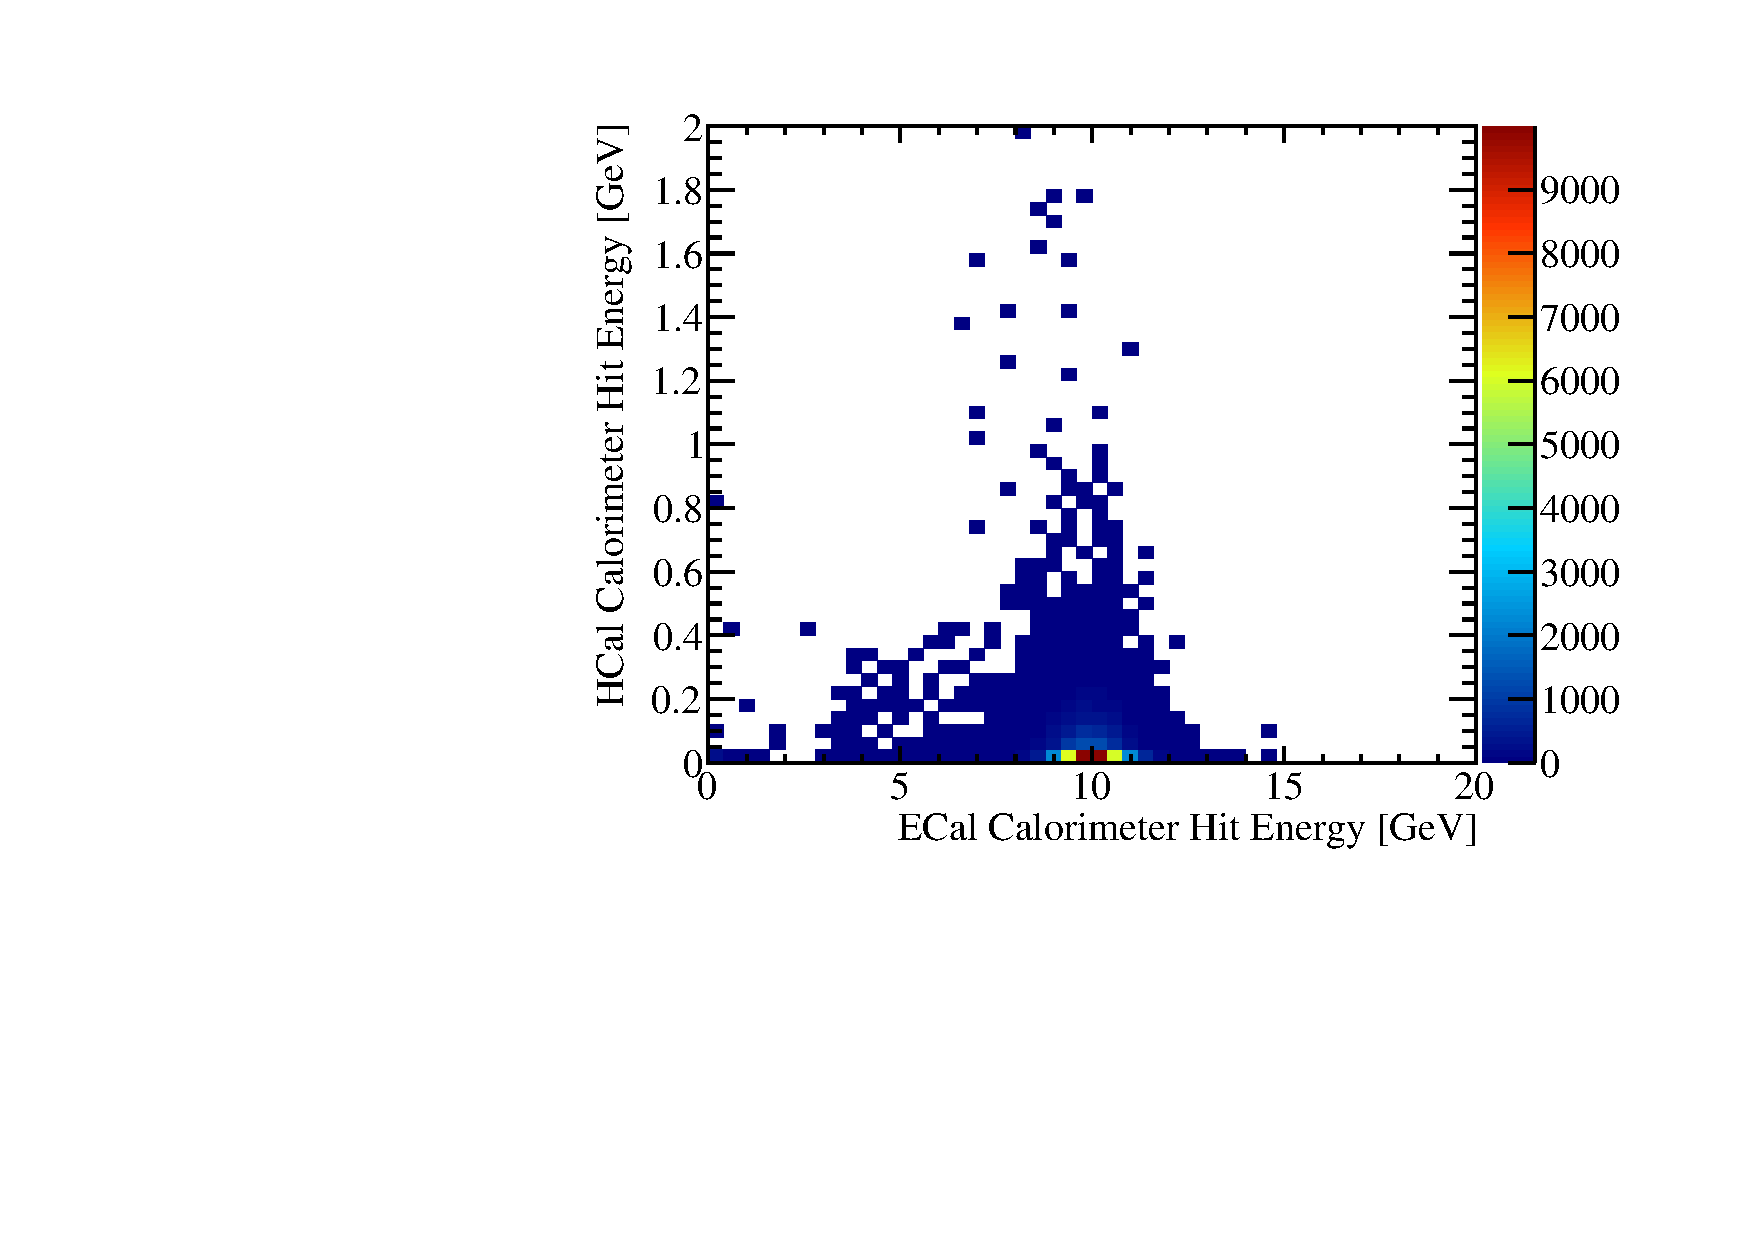
\includegraphics[width=0.5\textwidth]{EnergyEstimators/Plots/Calibration/Digitsation/ECal/ECalHCalPhotonSplit.pdf}
\caption[Sum of calorimeter hit energies in ECal and HCal for 10 GeV $\gamma$ events.]{Sum of calorimeter hit energies in ECal and HCal for 10 GeV $\gamma$ events.}
\label{fig:ecaldigiphotonsplit}
\end{figure}

Events are only considered in this analysis if they are confined to the ECal and to that extent cuts are applied ensuring that the sum of any reconstructed energy found outside the ECal is less than 1\% of $E_{MC}$ and that the $\text{cos}(\theta) < 0.95$ where $\theta$ is the polar angle of the $\gamma$.  $\gamma$ conversions are also vetoed from this event sample at this stage by requiring the reconstruction to give a single photon PFO.  The impact of these cuts on the sum of ECal calorimeter hit energies for the $E_{MC} = 10$ GeV $\gamma$ events is shown in figure \ref{fig:ecaldigiselection}.

\begin{figure}
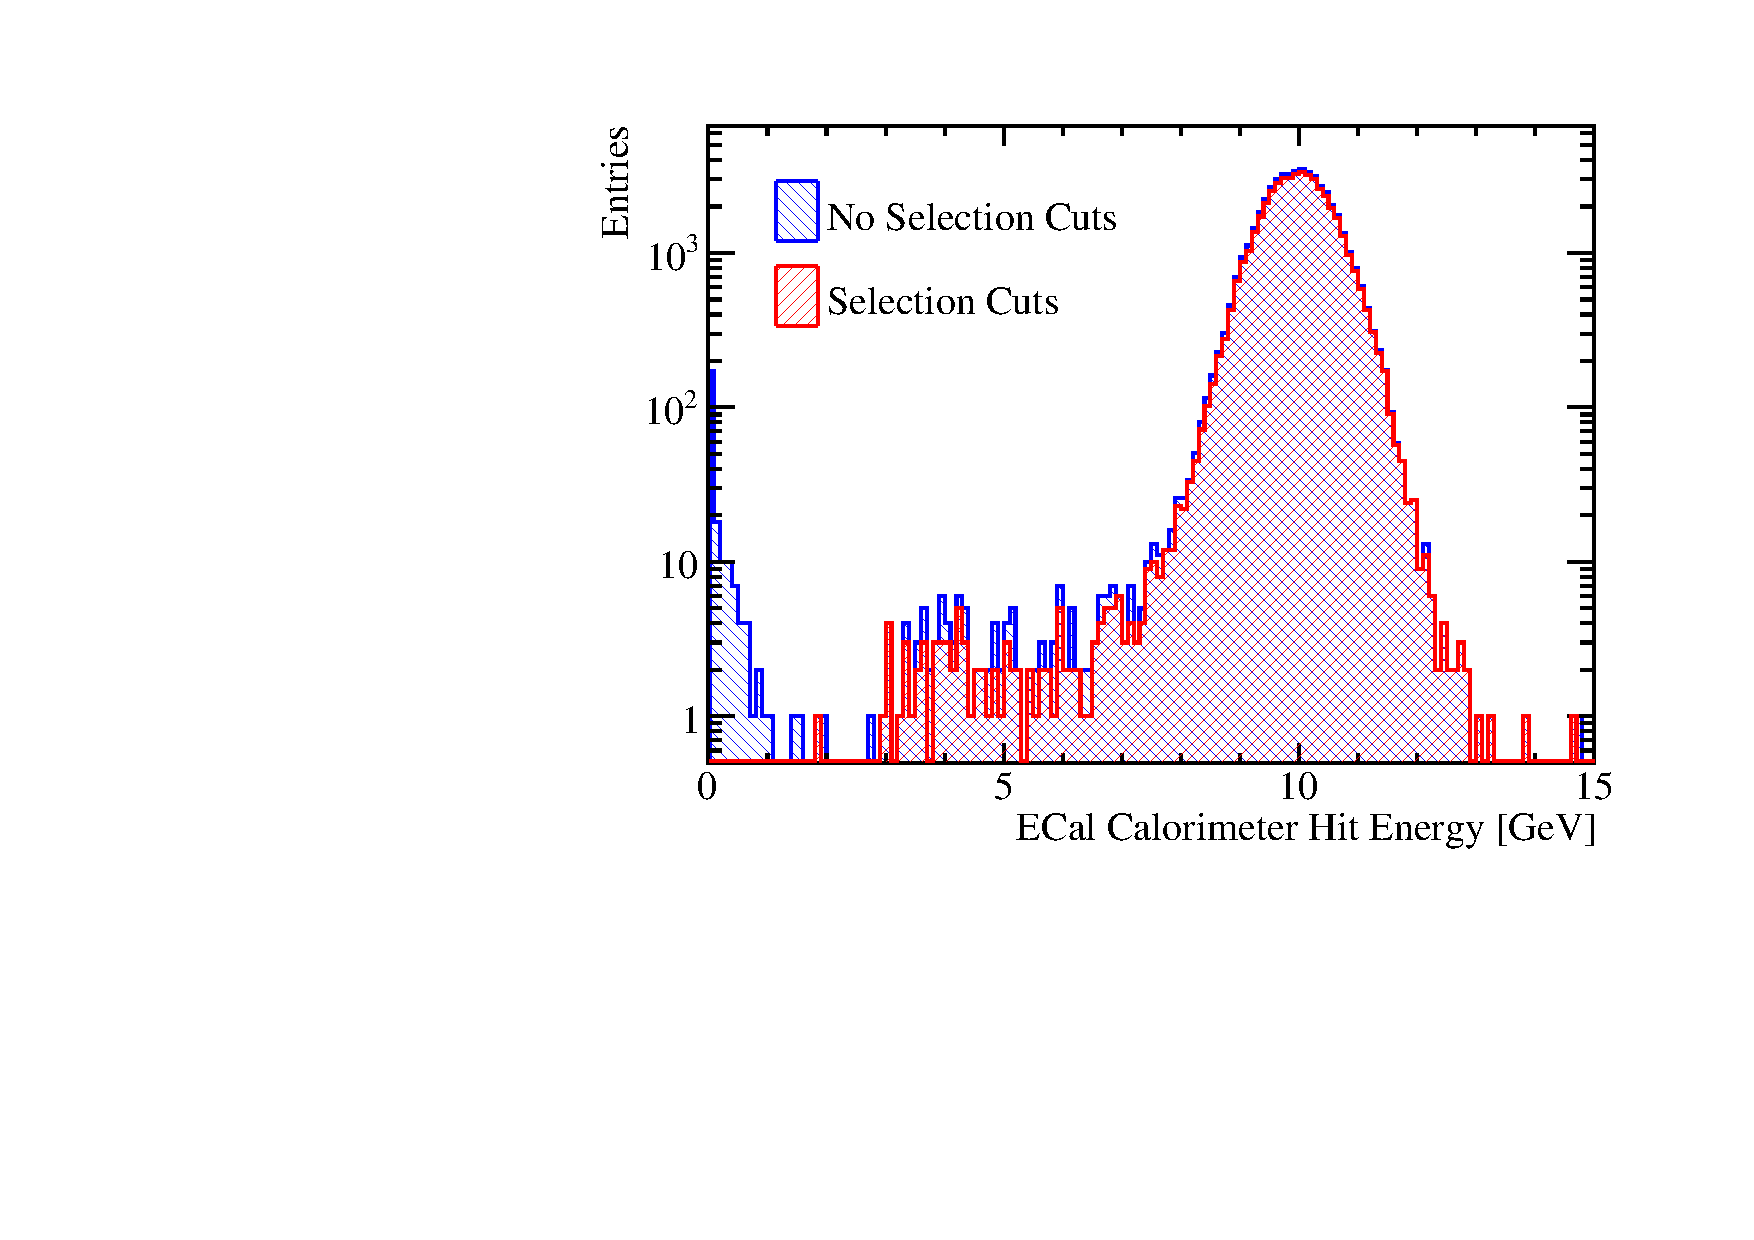
\includegraphics[width=0.5\textwidth]{EnergyEstimators/Plots/Calibration/Digitsation/ECal/DigitisationECalSelection.pdf}
\caption[Sum of the ECal calorimeter hit energies for 10 GeV $\gamma$ events with and without the selection cuts.]{Sum of the ECal calorimeter hit energies for 10 GeV $\gamma$ events with and without the selection cuts.}
\label{fig:ecaldigiselection}
\end{figure}

\begin{figure}
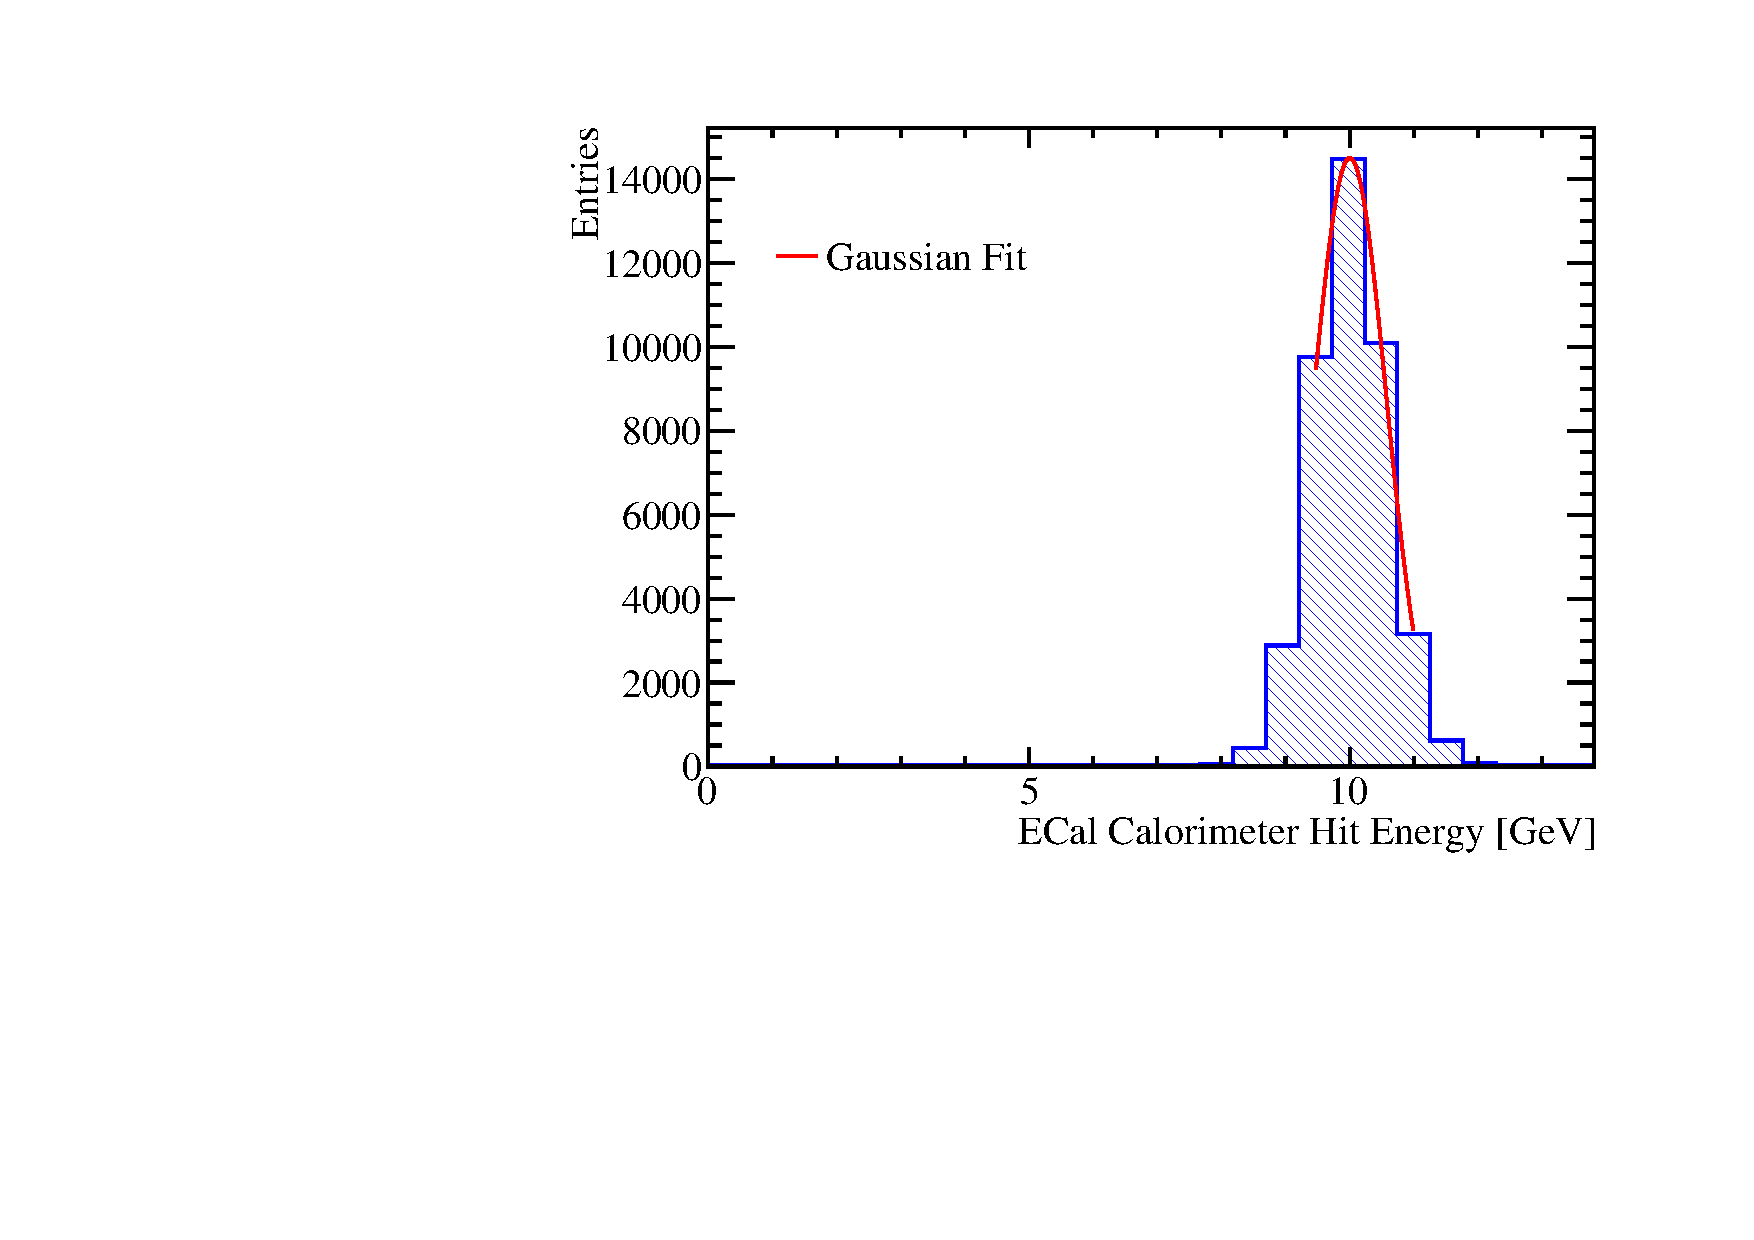
\includegraphics[width=0.5\textwidth]{EnergyEstimators/Plots/Calibration/Digitsation/ECal/DigitisationECalFit.pdf}
\caption[Gaussian fit to sum of the ECal calorimeter hit energies for 10 GeV $\gamma$ events with selection cuts.]{Gaussian fit to sum of the ECal calorimeter hit energies for 10 GeV $\gamma$ events with selection cuts.}
\label{fig:ecaldigifit}
\end{figure}

The calibration procedure is iterative and begins with the simulated single $\gamma$ events using a trial calibration, with digitisation constant in the ECal $\alpha^{0}_{\text{ECal}}$, which may not be ideal.  Then the distribution of the sum of calorimeter hit energies within the ECal is produced for events passing the selection cuts using, as shown in figure \ref{fig:ecaldigiselection}.  For an ideal calorimeter this distribution should be Gaussian, as was described in section CALORIMETER CHAPTER.  Therefore, a Gaussian fit is applied to this distribution and the mean, $E_{\text{Fit}}$, extracted.  In an attempt to remove the effect of any outliers in this distribution, the fit is applied to the range of data with the smallest root mean square that contains at least 90 \% of the data.  An example of such a fit is shown in figure \ref{ig:ecaldigifit}.  In the case of perfect calibration the mean of this fit would be equal $E_{MC}$ and it is assumed that any deviation between the two is due to inaccurate calibration.  To correct for any such deviation the digitisation constant from the trial calibration, $\alpha^{0}_{\text{ECal}}$, is rescaled by the ratio of the $E_{MC}$ to $E_{\text{Fit}}$.

\begin{equation}
\alpha^{0}_{\text{ECal}} \rightarrow \alpha_{\text{ECal}} = \alpha^{0}_{\text{ECal}} \times \frac{E_{MC}}{E_{Fit}}
\end{equation}

This procedure is then repeated until the $E_{\text{Fit}}$ falls within a chosen tolerance of $E_{\text{MC}}$.  The tolerance that was applied here is that $|E_{\text{Fit}} - E_{\text{MC}}| < E_{\text{MC}} \times 5 \%$.  The binning for the fitted histogram is chosen such that the bin width is equal to the desired tolerance on $E_{\text{Fit}}$ e.g. $E_{\text{MC}} \times 5 \% = 0.5$ GeV.  This tolerance is somewhat large, however, it is tight enough to ensure successful application of PFA.  It should also be emphasised that the PFO energies used in downstream analyses have the electromagnetic and hadronic energy scale corrections applied and these are calibrated to a much tighter accuracy.

%========================================================================================

\subsubsection{HCal Digitisation}
\label{sec:hcaldigi}
The calibration for the digitisation in the HCal proceeds in a similar manor to that described for the ECal with a few key differences.  This calibration uses $K^{0}_{L}$ events at $E_{MC} = 20$ GeV as these neutral hadrons will deposit the bulk of their energy in the HCal.  The higher energy is used to create larger particle showers and sample deeper into the calorimeters.  

As the $K^{0}_{L}$ samples have to pass through the ECal before arriving at the HCal and as the ECal contains $\approx 1 \lambda_{I}$, some of the particles begin showering in the ECal, as shown by figure \ref{fig:hcaldigikaonsplit}.  These events are unsuitable for calibration as rescaling $\alpha^{0}_{\text{HCal}}$ does not lead to a linear rescaling in the mean of $E_{\text{Fit}}$.  This issue is resolve by applying selection cuts to select events that deposit the bulk of their energy in the HCal.  

\begin{figure}
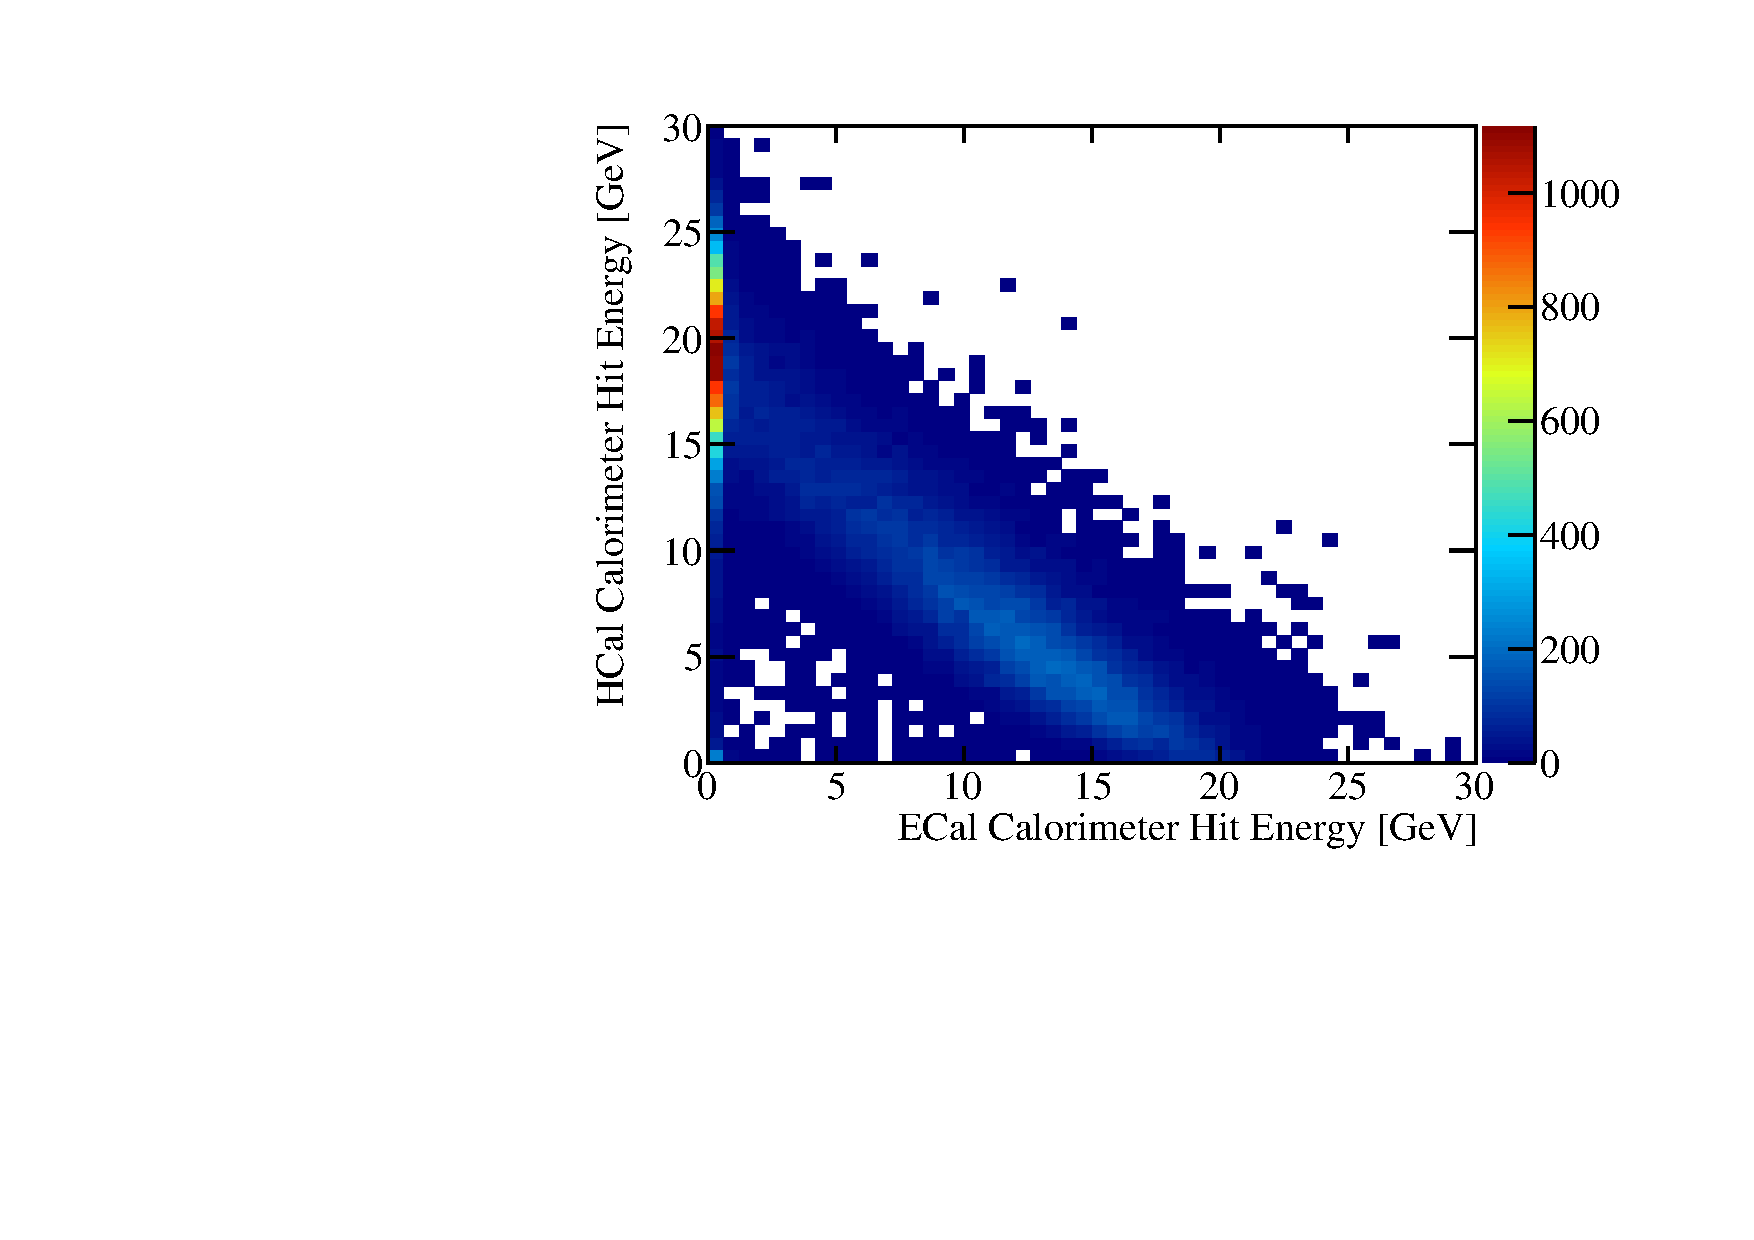
\includegraphics[width=0.5\textwidth]{EnergyEstimators/Plots/Calibration/Digitsation/HCal/ECalHCalKaon0LSplit.pdf}
\caption[Sum of calorimeter hit energies in ECal and HCal for 20 GeV $K^{0}_{L}$ events.]{Sum of calorimeter hit energies in ECal and HCal for 20 GeV $K^{0}_{L}$ events.}
\label{fig:hcaldigikaonsplit}
\end{figure}

Events are only considered in this analysis if a single neutral hadron PFO is reconstruction, the sum of any reconstructed energy found outside the HCal is less than 5\% of $E_{MC}$ and the last layer of the HCal where energy is deposited is in the first 90\% of the HCal.  The cut on the last HCal layer where energy is deposited is applied to veto events that shower late in the HCal and deposit a significant amount of energy in the uninstrumented coil region of the detector.  The impact of these cuts on the sum of HCal calorimeter hit energies for the $E_{MC} = 20$ GeV $K^{0}_{L}$ events is shown in figure \ref{fig:hcaldigiselection}.

\begin{figure}
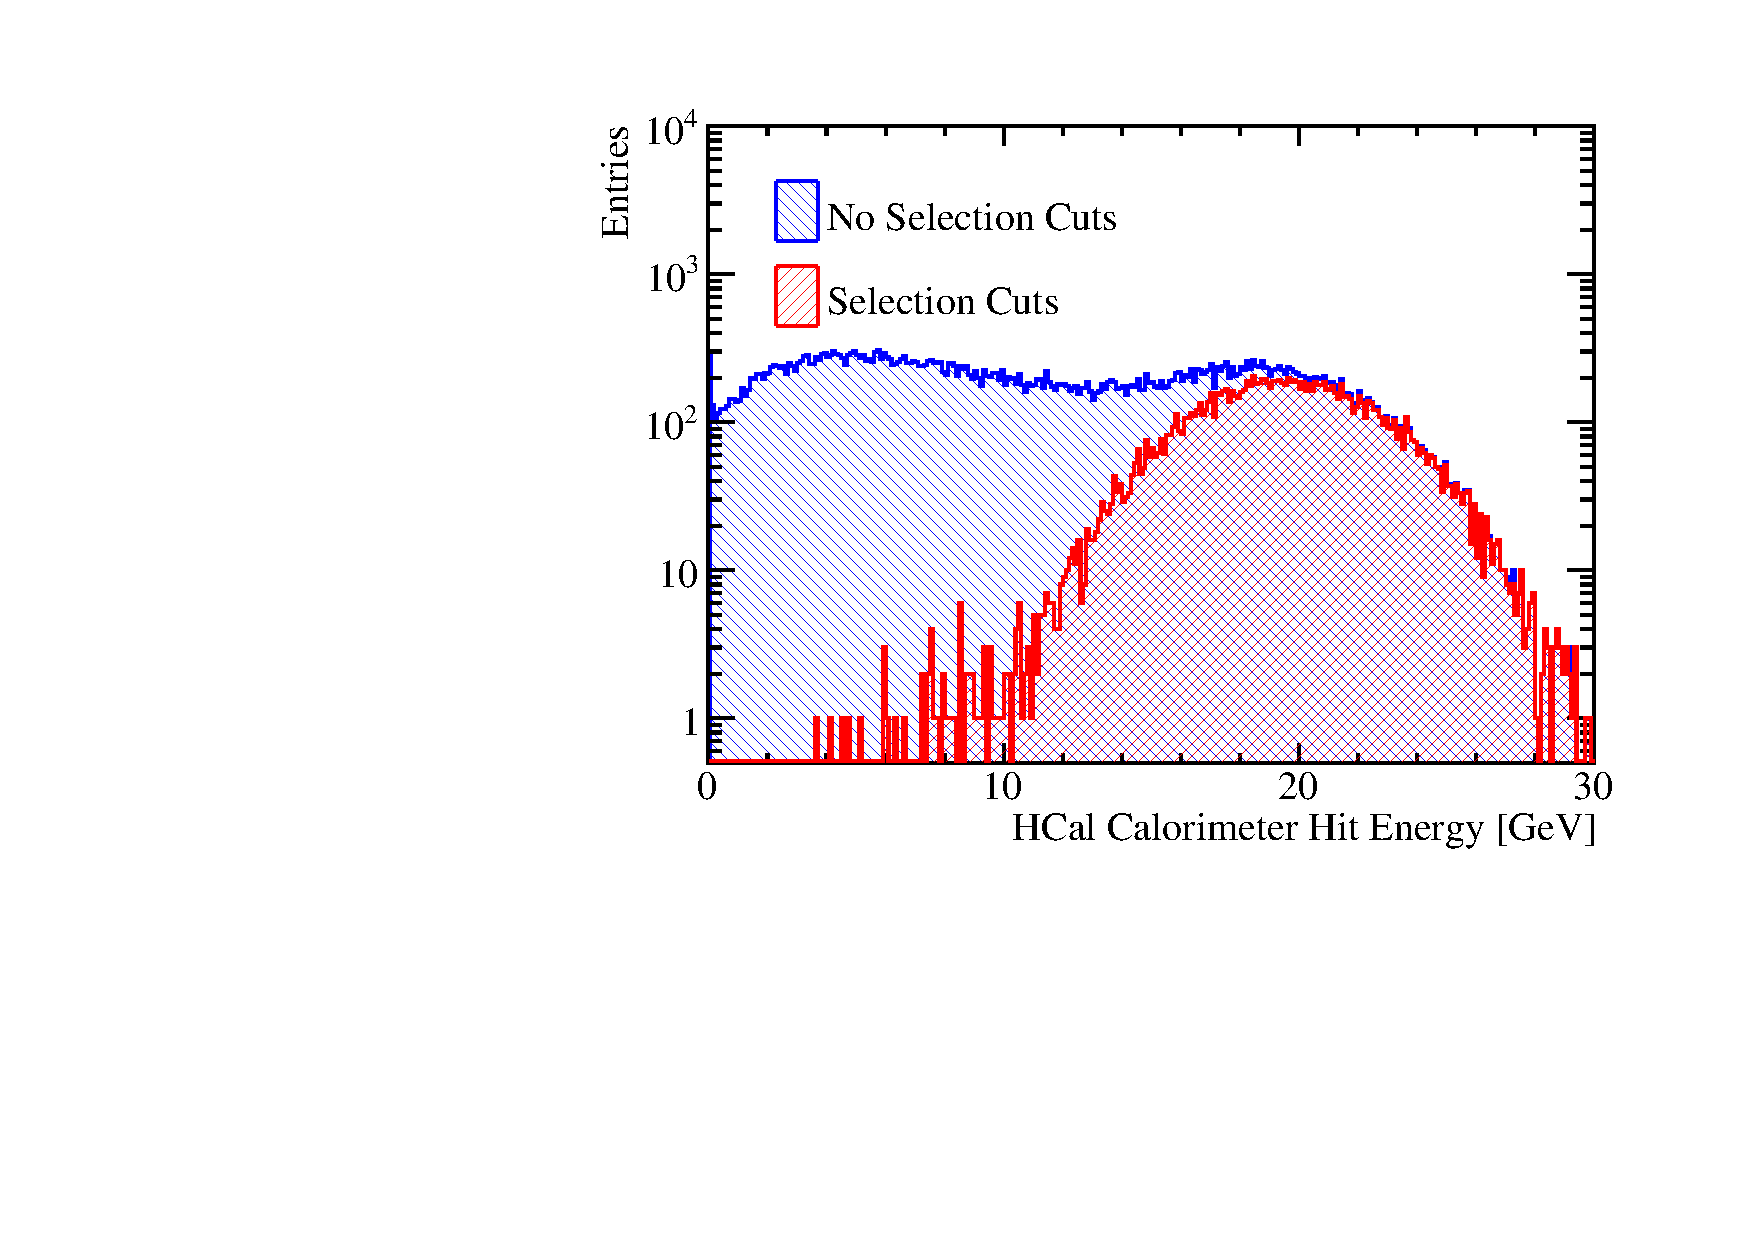
\includegraphics[width=0.5\textwidth]{EnergyEstimators/Plots/Calibration/Digitsation/HCal/DigitisationHCalSelection.pdf}
\caption[Sum of the HCal calorimeter hit energies for a 20 GeV $K^{0}_{L}$ events with and without the selection cuts.]{Sum of the HCal calorimeter hit energies for a 20 GeV $K^{0}_{L}$ events with and without the selection cuts.}
\label{fig:hcaldigiselection}
\end{figure}

There are two HCal digitisation constants used in the detector simulation, one applied for the HCal barrel and another for the HCal EndCap.  This is to account for differences in hadronic shower dynamics that exist due to a variety of reasons such as differing magnetic field configurations in the Barrel and EndCap.  Both parameters are calibrated in the same manor, but have different cuts on $\theta$, the polar angle of the $K^{0}_{L}$.  For the Barrel region of the HCal $0.2 < \text{cos}(\theta) < 0.6$, while for the EndCap $0.8 < \text{cos}(\theta) < 0.9$.  These angular cuts are conservative to account for the transverse profile of the hadronic showers and ensure that they are confined to the relevant sub-detector.

Using these cuts the calibration procedure for the digitisation of the HCal Barrel and EndCap proceeds in the same manor as was described for the ECal, the details of which can be found in section \ref{sec:ecaldigi}, and examples of the Gaussian fits applied to the sum of the calorimeter hit energies in the HCal Barrel and EndCap can be found in figure \ref{fig:hcaldigifit}. 

\begin{figure}
\subfloat[HCal Barrel.]{\label{fig:hcaldigibarrel}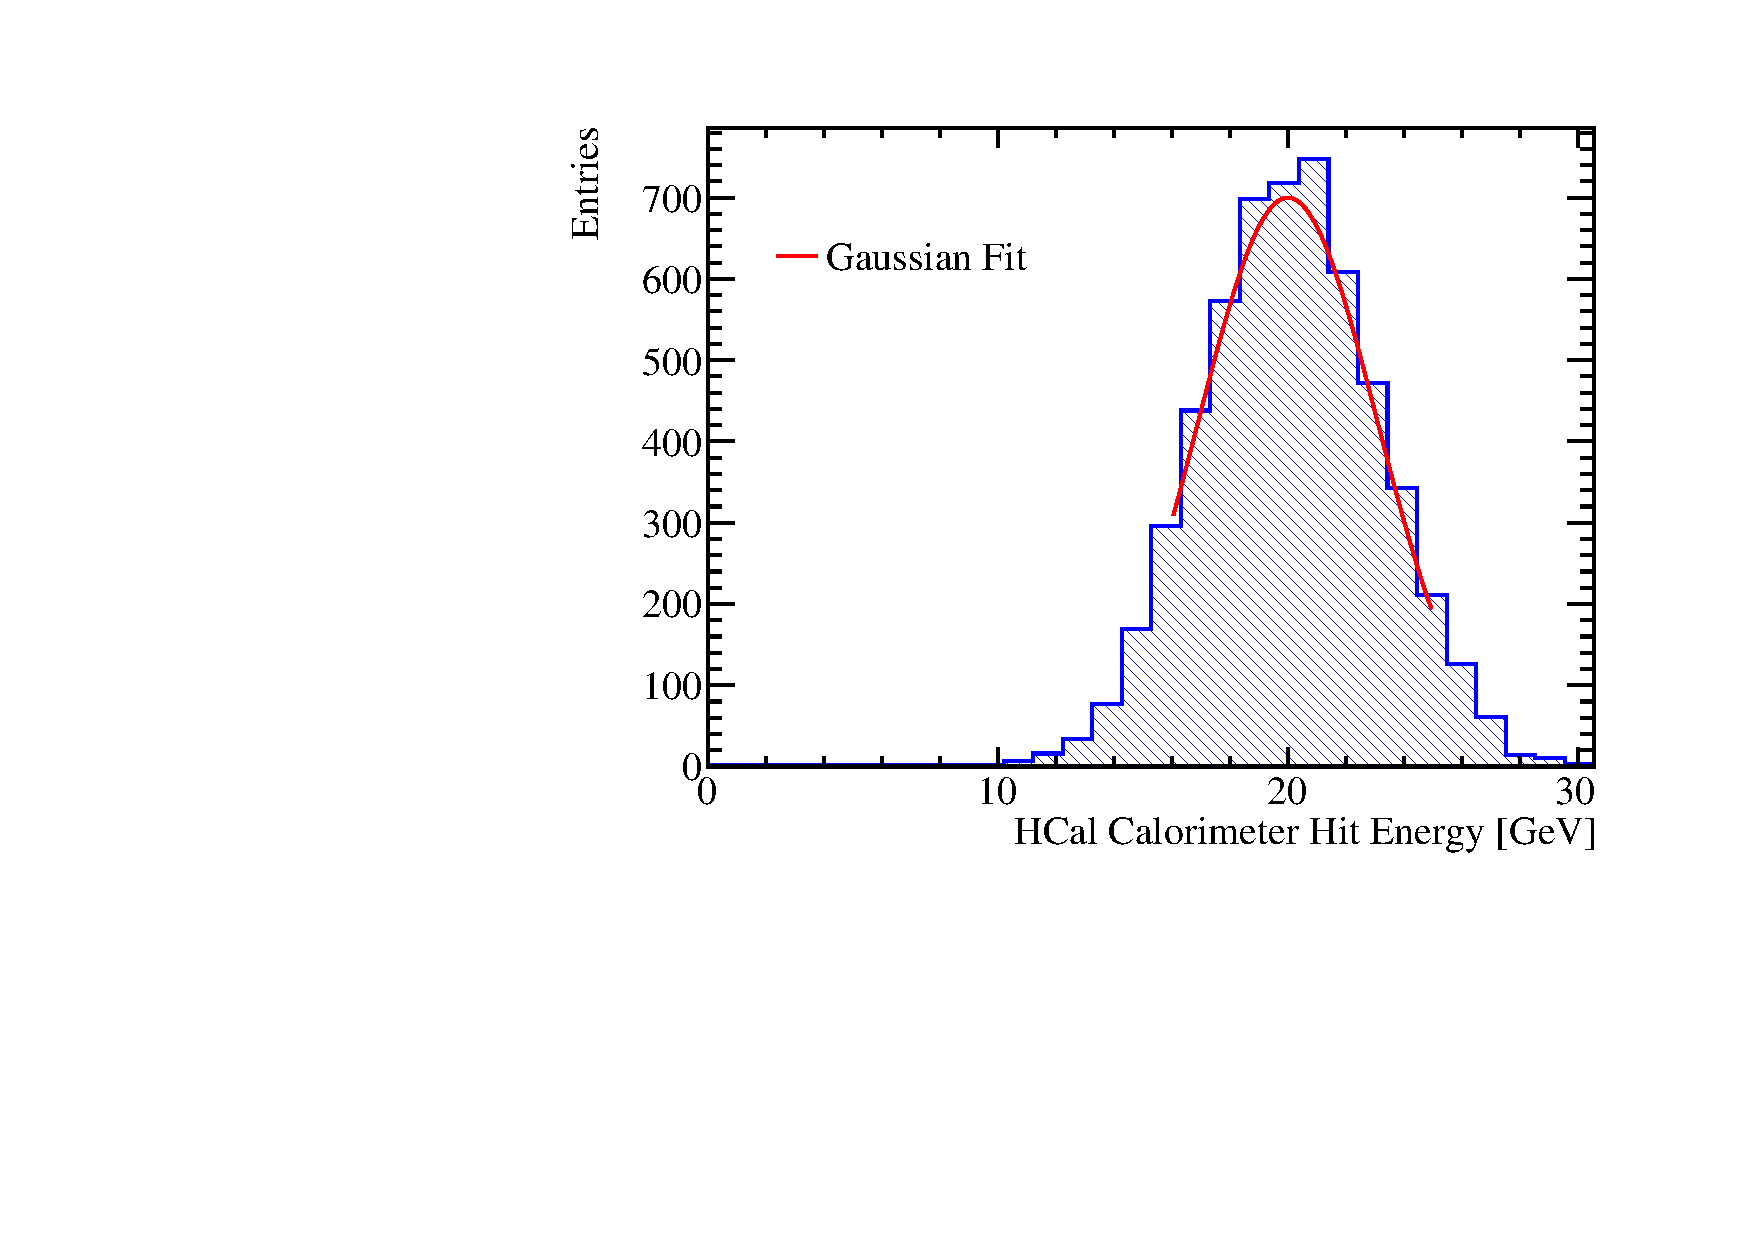
\includegraphics[width=0.5\textwidth]{EnergyEstimators/Plots/Calibration/Digitsation/HCal/DigitisationHCalBarrelFit.pdf}}
\subfloat[HCal EndCap.]{\label{fig:hcaldigiendcap}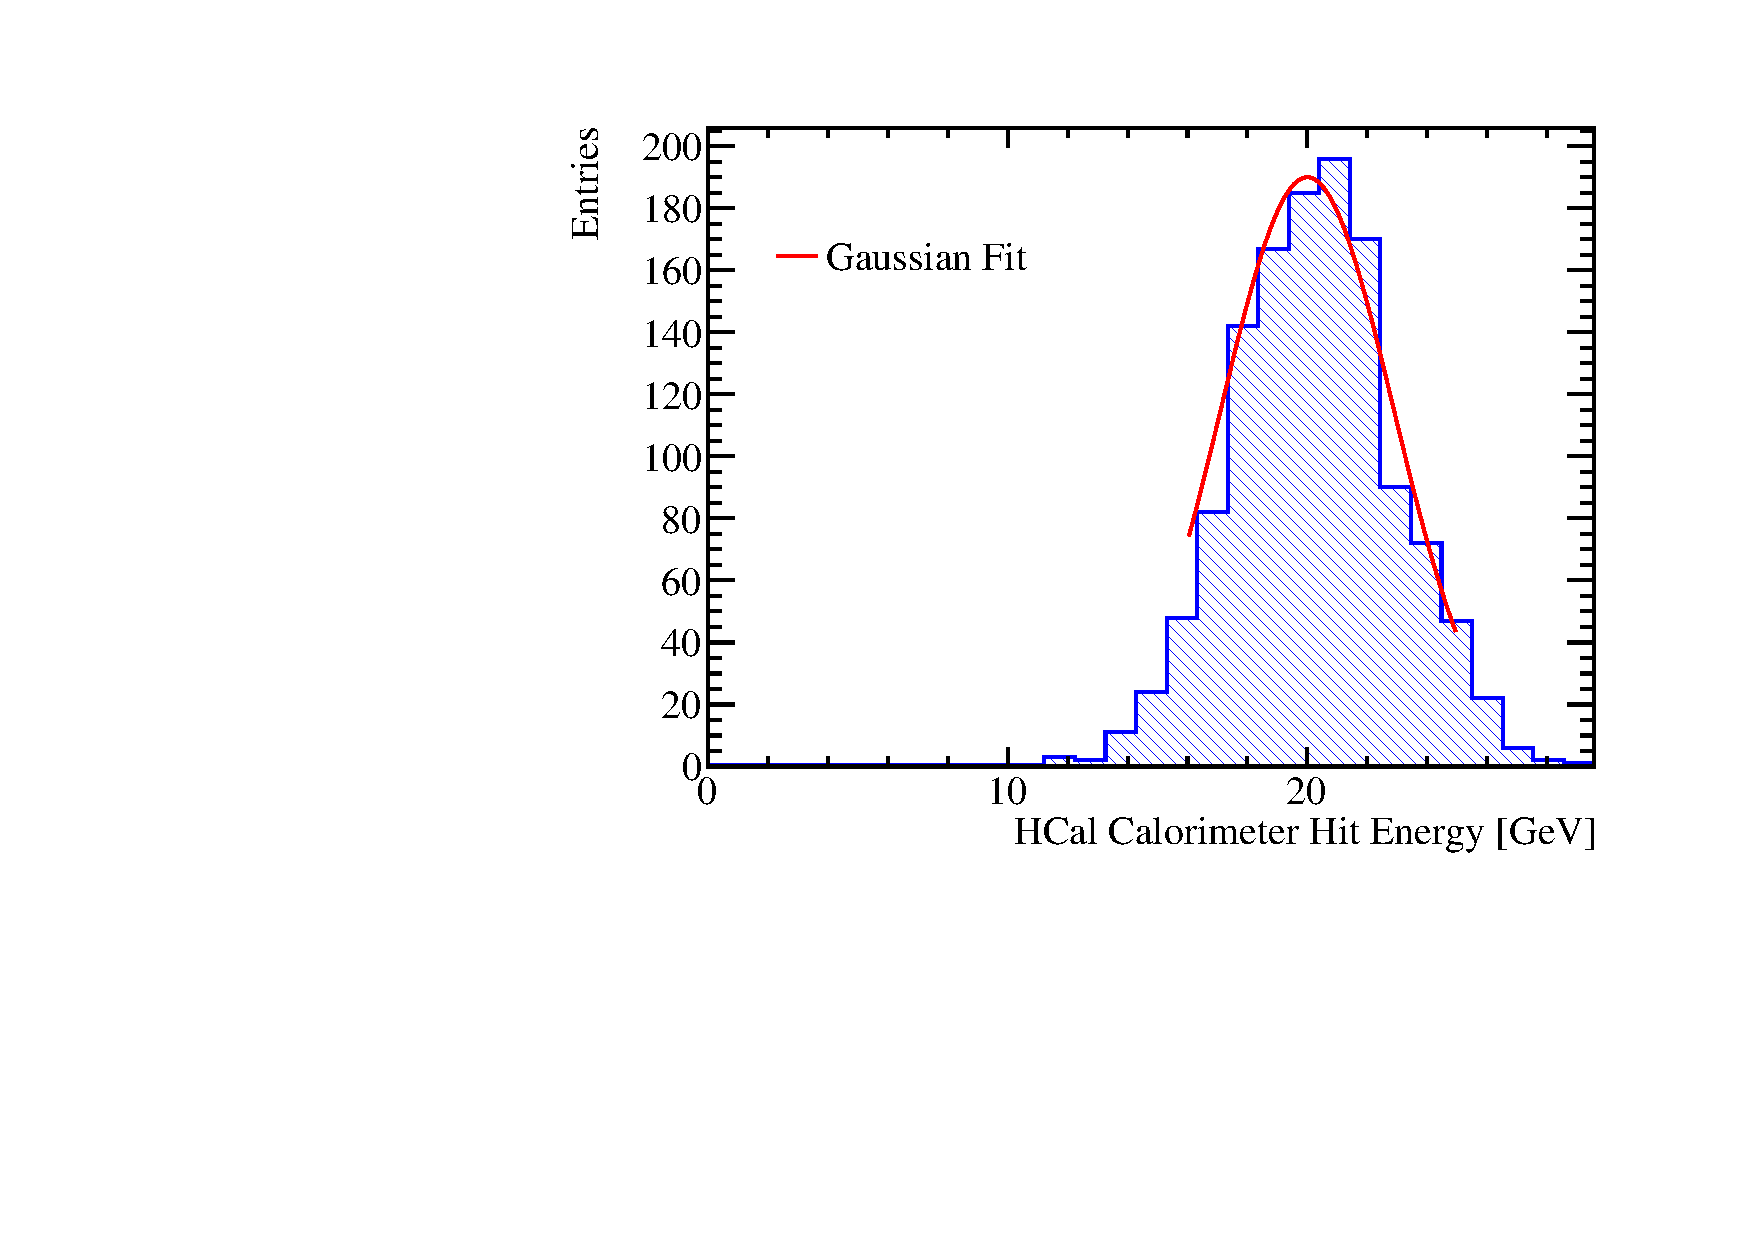
\includegraphics[width=0.5\textwidth]{EnergyEstimators/Plots/Calibration/Digitsation/HCal/DigitisationHCalEndCapFit.pdf}}
\caption[Gaussian fit to sum of the HCal calorimeter hit energies for 20 GeV $K^{0}_{L}$ events with selection cuts.]{Gaussian fit to sum of the HCal calorimeter hit energies for 20 GeV $K^{0}_{L}$ events with selection cuts.}
\label{fig:hcaldigifit}
\end{figure}

%========================================================================================

\subsubsection{HCal Ring Digitisation}
\label{sec:hcalringdigi}
The HCal ring also has an independent digitisation constant for the same reasons that the Barrel and EndCap constants differ.  The procedure used to calibrate this constant has to differ from that presented in section \ref{sec:hcaldigi} as it is unfeasible, due to the depth of the ring, to produce events that are wholly contained within it.  Fortunately, the size of the HCal ring means that it will play a minimal role in the reconstruction, so precise calibration is not crucial.  To ensure that the calibration is approximately correct for the HCal Ring, $\alpha_{\text{HCal Ring}}$ is assumed to equal $\alpha_{\text{HCal EndCap}}$ multiplied by several factors designed to accounts for changes in the active layer thickness, absorber layer thickness and the MIP response between the HCal EndCap and Ring.  In detail:

\begin{equation}
\alpha_{\text{HCal Ring}} = \alpha_{\text{HCal EndCap}} \times \frac{\langle \text{cos}(\theta_\text{EndCap}) \rangle}{\langle \text{cos}(\theta_\text{Ring}) \rangle} \times \frac{P_\text{EndCap} }{P_\text{Ring} } \times \frac{L^{Absorber}_\text{EndCap}}{L^{Absorber}_\text{Ring} } \times \frac{L^{Active}_\text{Ring}}{L^{Active}_\text{EndCap}}
\end{equation}

where $\theta$ is the incident angle of the incoming particle to the calorimeter cells determined using the 20 GeV $K^{0}_{L}$ events, $L^{Active}$ is the active layer thickness, $L^{Absorber}$ is the absorber layer thickness and $P$ is the position of the MIP peak in the distribution of active layer cell energies, corrected so that the particles appear normally incident, using 10 GeV $\mu^{-}$ events.  Details on how $P$ is determined can be found in section \ref{sec:mipresponse}.

%========================================================================================

\subsection{MIP Scale Setting}
\label{sec:mipresponse}
The response of the various sub-detectors to a MIP has to be determined for both the digitisation processor and for PandoraPFA as both apply cuts in units of MIP response.  The digitiser applies cuts related to the electronic readout range of the various active layer technology options and applies thresholds on the minimum active layer energy for the creation of calorimeter hits, while PandoraPFA applies cuts that would veto noise that would be present in a real detector.  Both these MIP responses, while intrinsically linked, have to be calculated separately as the digitiser requires the MIP peak definition from the active layer cell energies while, PandoraPFA requires the definition from the full cell, active and absorber layer, energies.  In these studies a MIP was defined as a 10 GeV $\mu^{-}$ \cite{Bichsel:2004ej} and there were no selection cuts applied to this sample.  

For the digitiser the MIP scale was defined as the, non-zero, peak in the distribution of the active layer calorimeter cell energies for normally incident $\mu^{-}$ as shown in figure \ref{fig:digitisermip}.  This distribution was produced using a sample of $\mu^{-}$ events that are spatially isotropic about the impact point.  A direction correction factor, $\text{cos}(\theta)$ where $\theta$ is the indecent angle of the incoming $\mu^{-}$ to the calorimeter cell, was applied to the active layer cell energies to generate the effect of having normally incident $\mu^{-}$.  

\begin{figure}
\subfloat[ECal.]{\label{fig:digitisermipecal}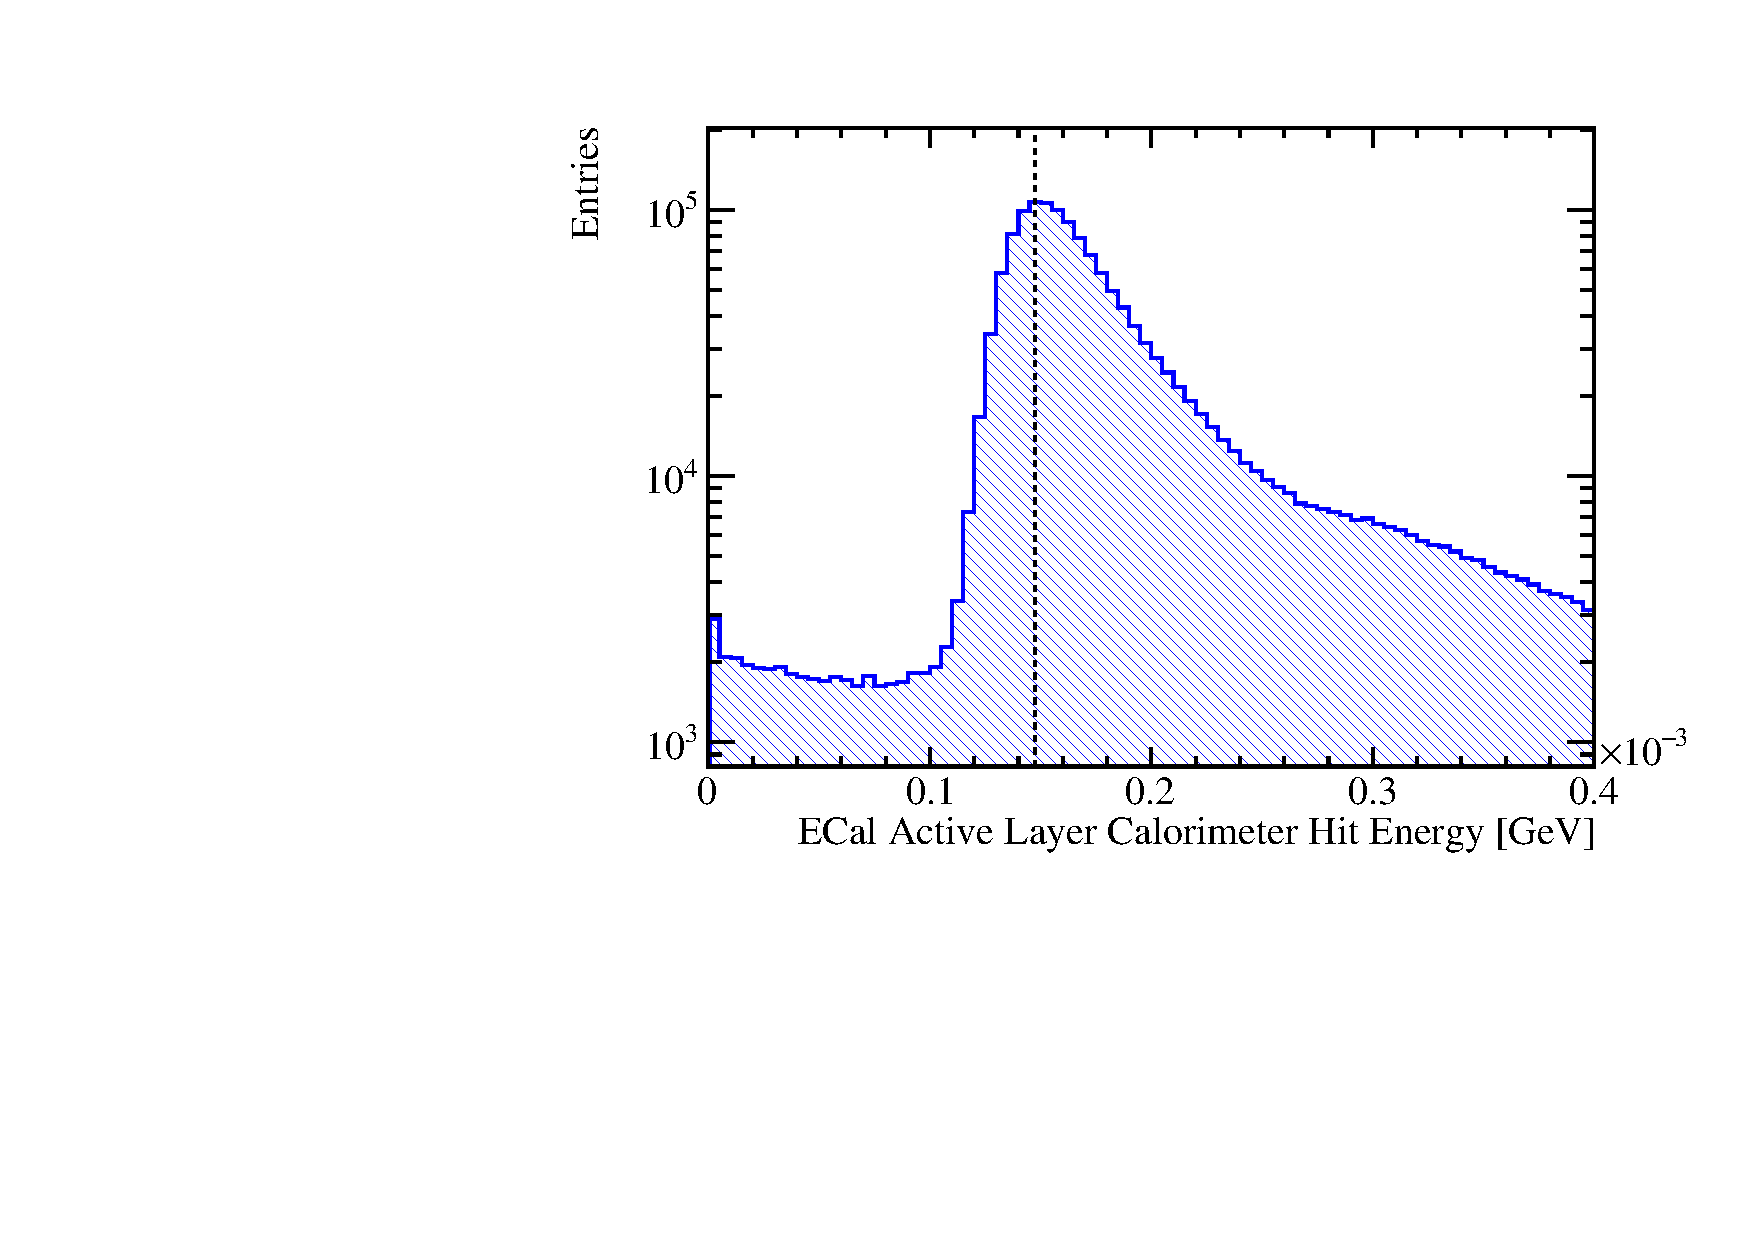
\includegraphics[width=0.5\textwidth]{EnergyEstimators/Plots/Calibration/MIPScale/Digitiser/MIPScaleDigitiserECal.pdf}}
\subfloat[HCal Barrel.]{\label{fig:digitisermiphcalbarrel}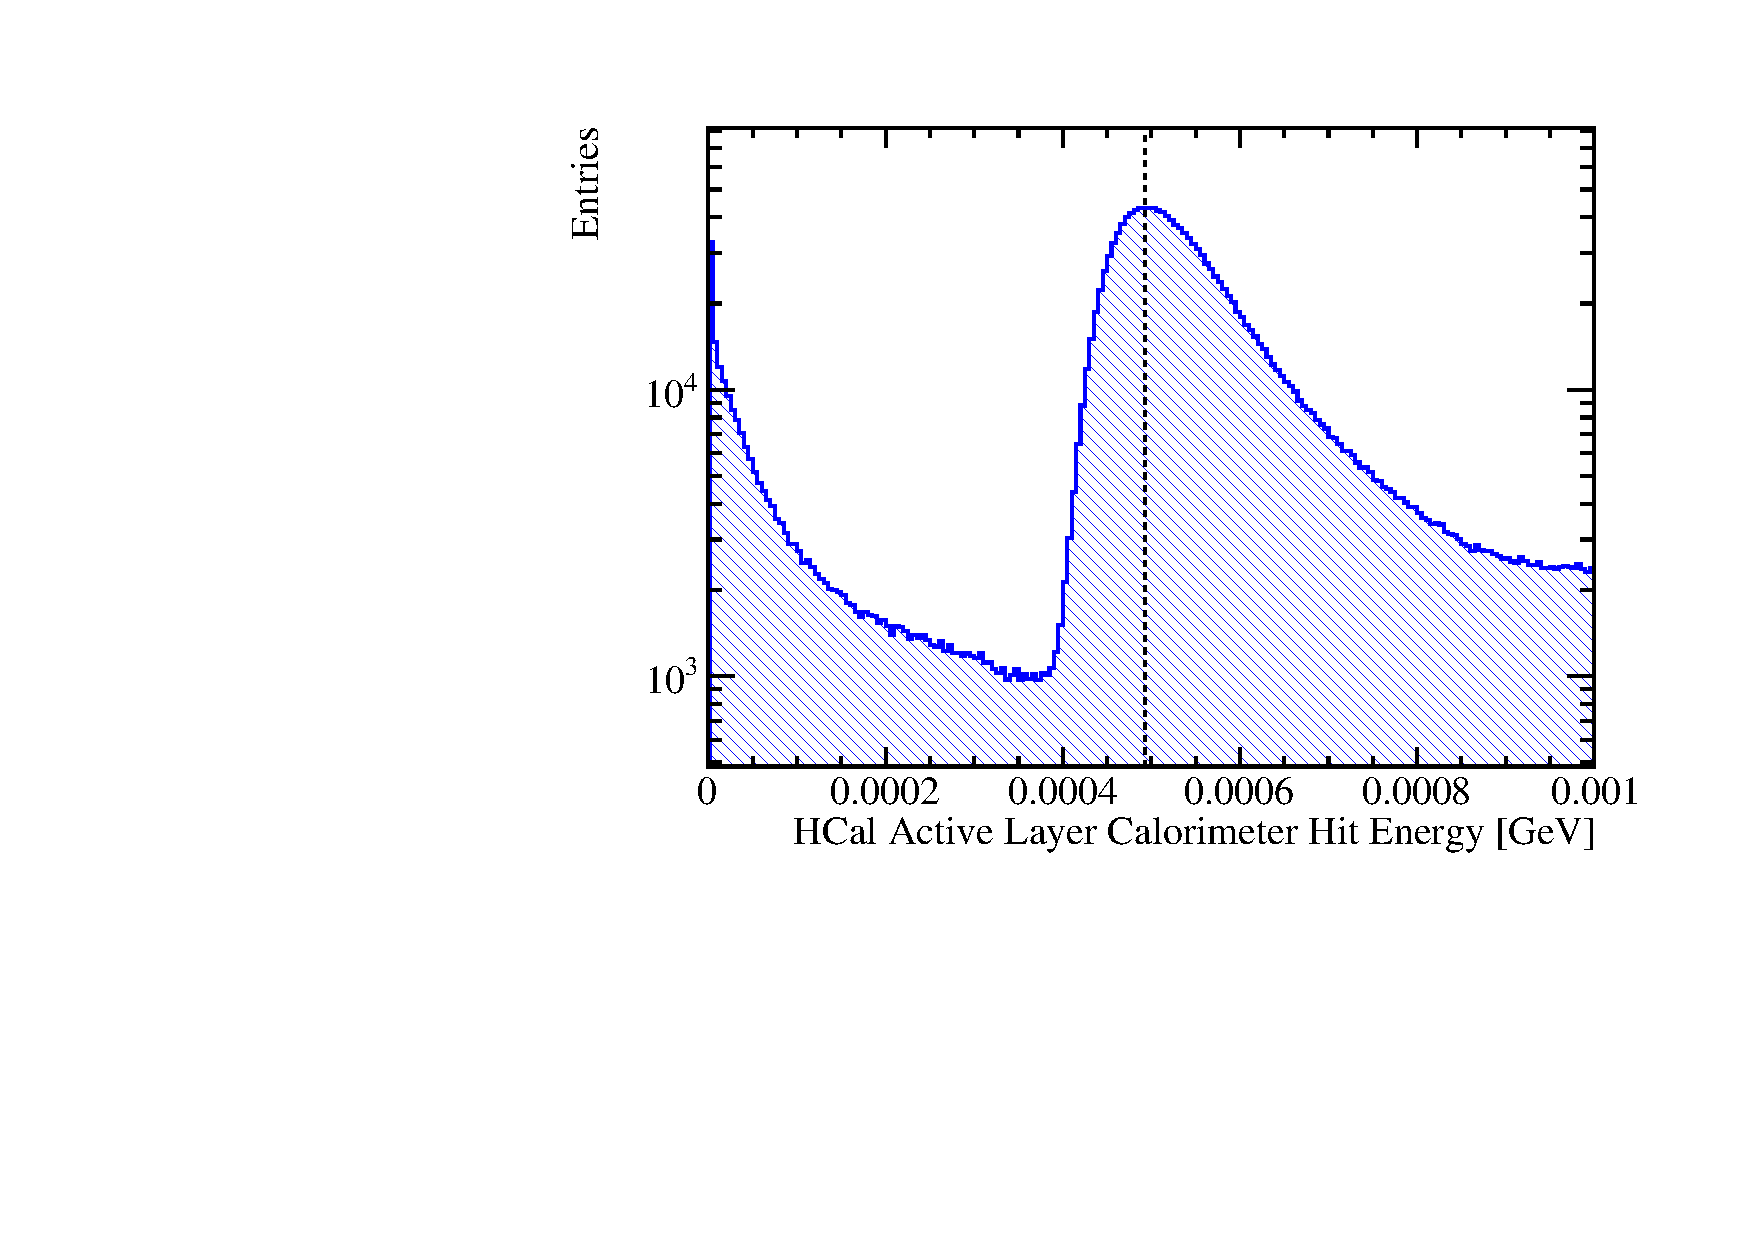
\includegraphics[width=0.5\textwidth]{EnergyEstimators/Plots/Calibration/MIPScale/Digitiser/MIPScaleDigitiserHCalBarrel.pdf}} \\
\subfloat[HCal EndCap.]{\label{fig:digitisermiphcalendcap}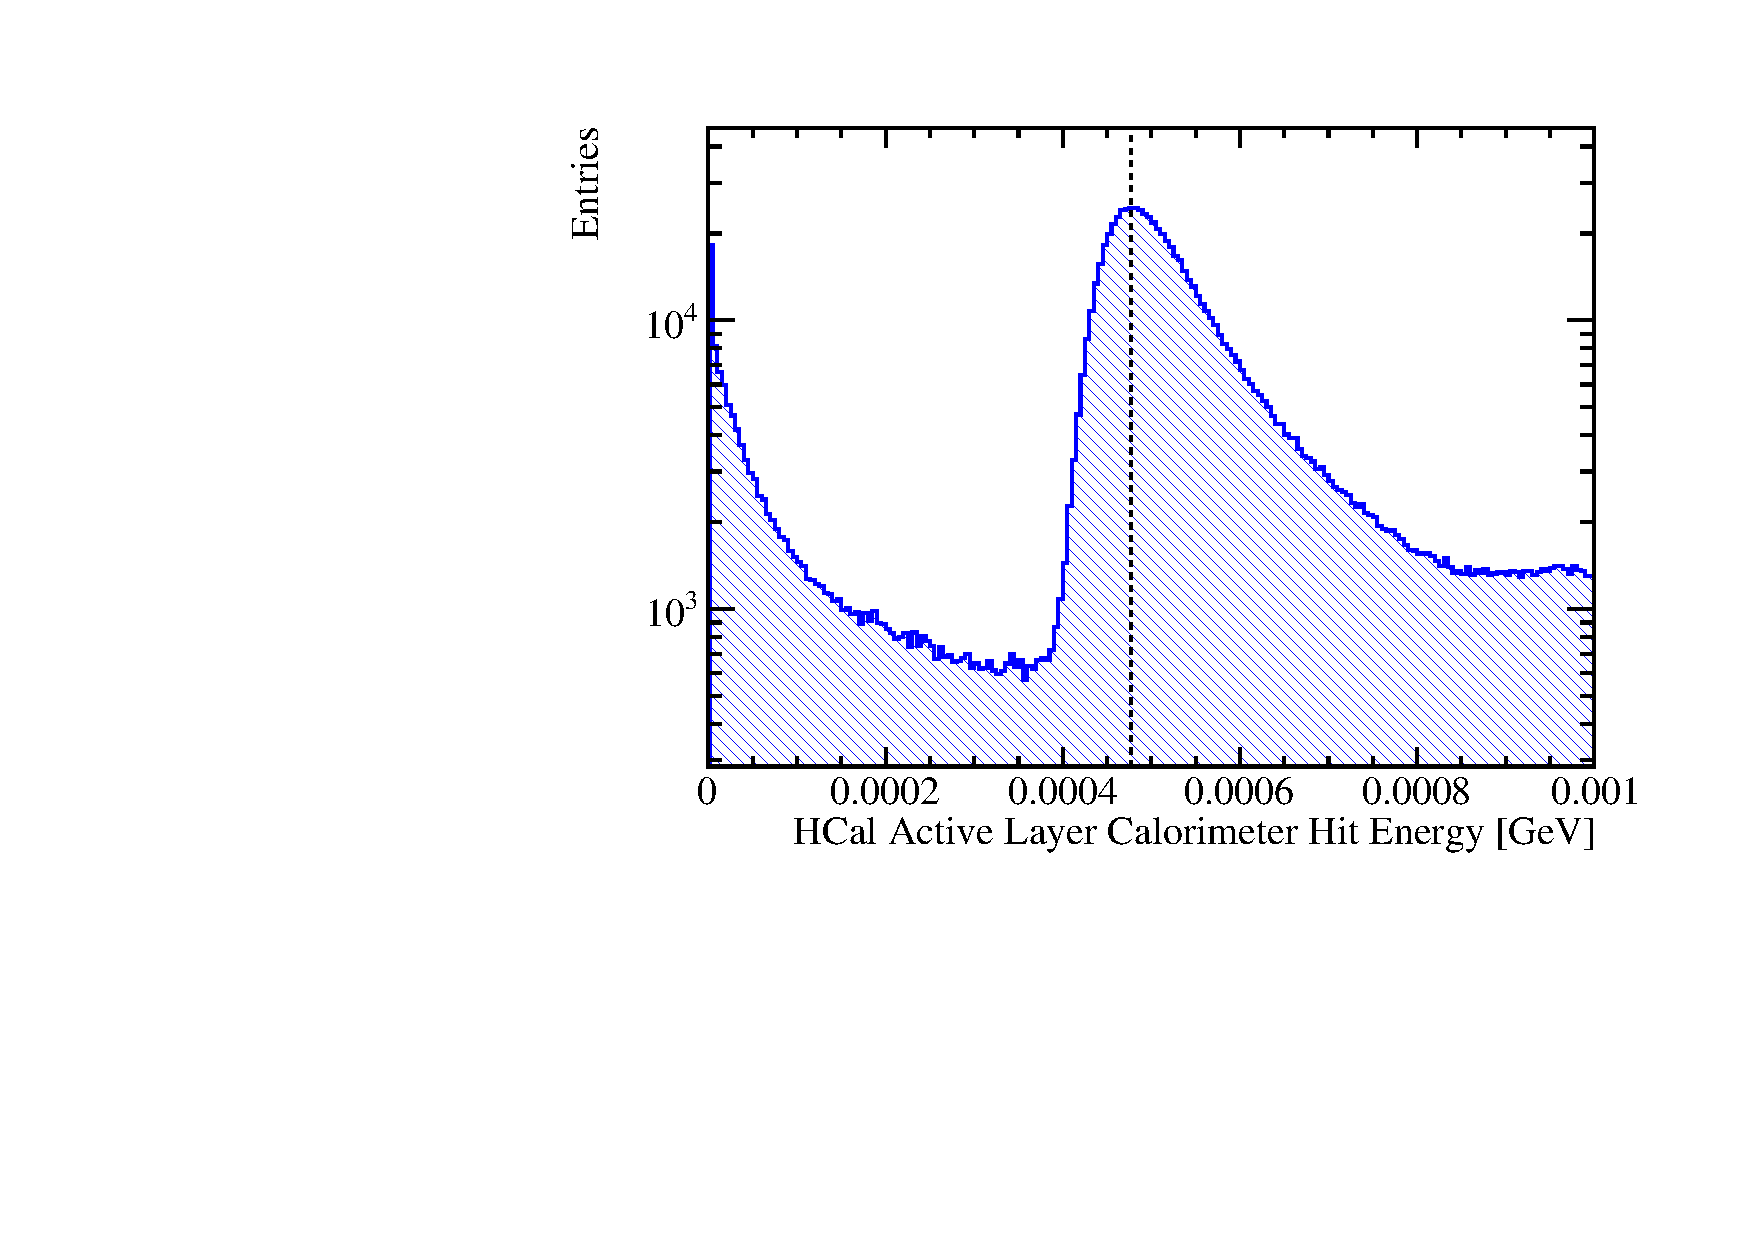
\includegraphics[width=0.5\textwidth]{EnergyEstimators/Plots/Calibration/MIPScale/Digitiser/MIPScaleDigitiserHCalEndCap.pdf}}
\subfloat[HCal Ring.]{\label{fig:digitisermiphcalring}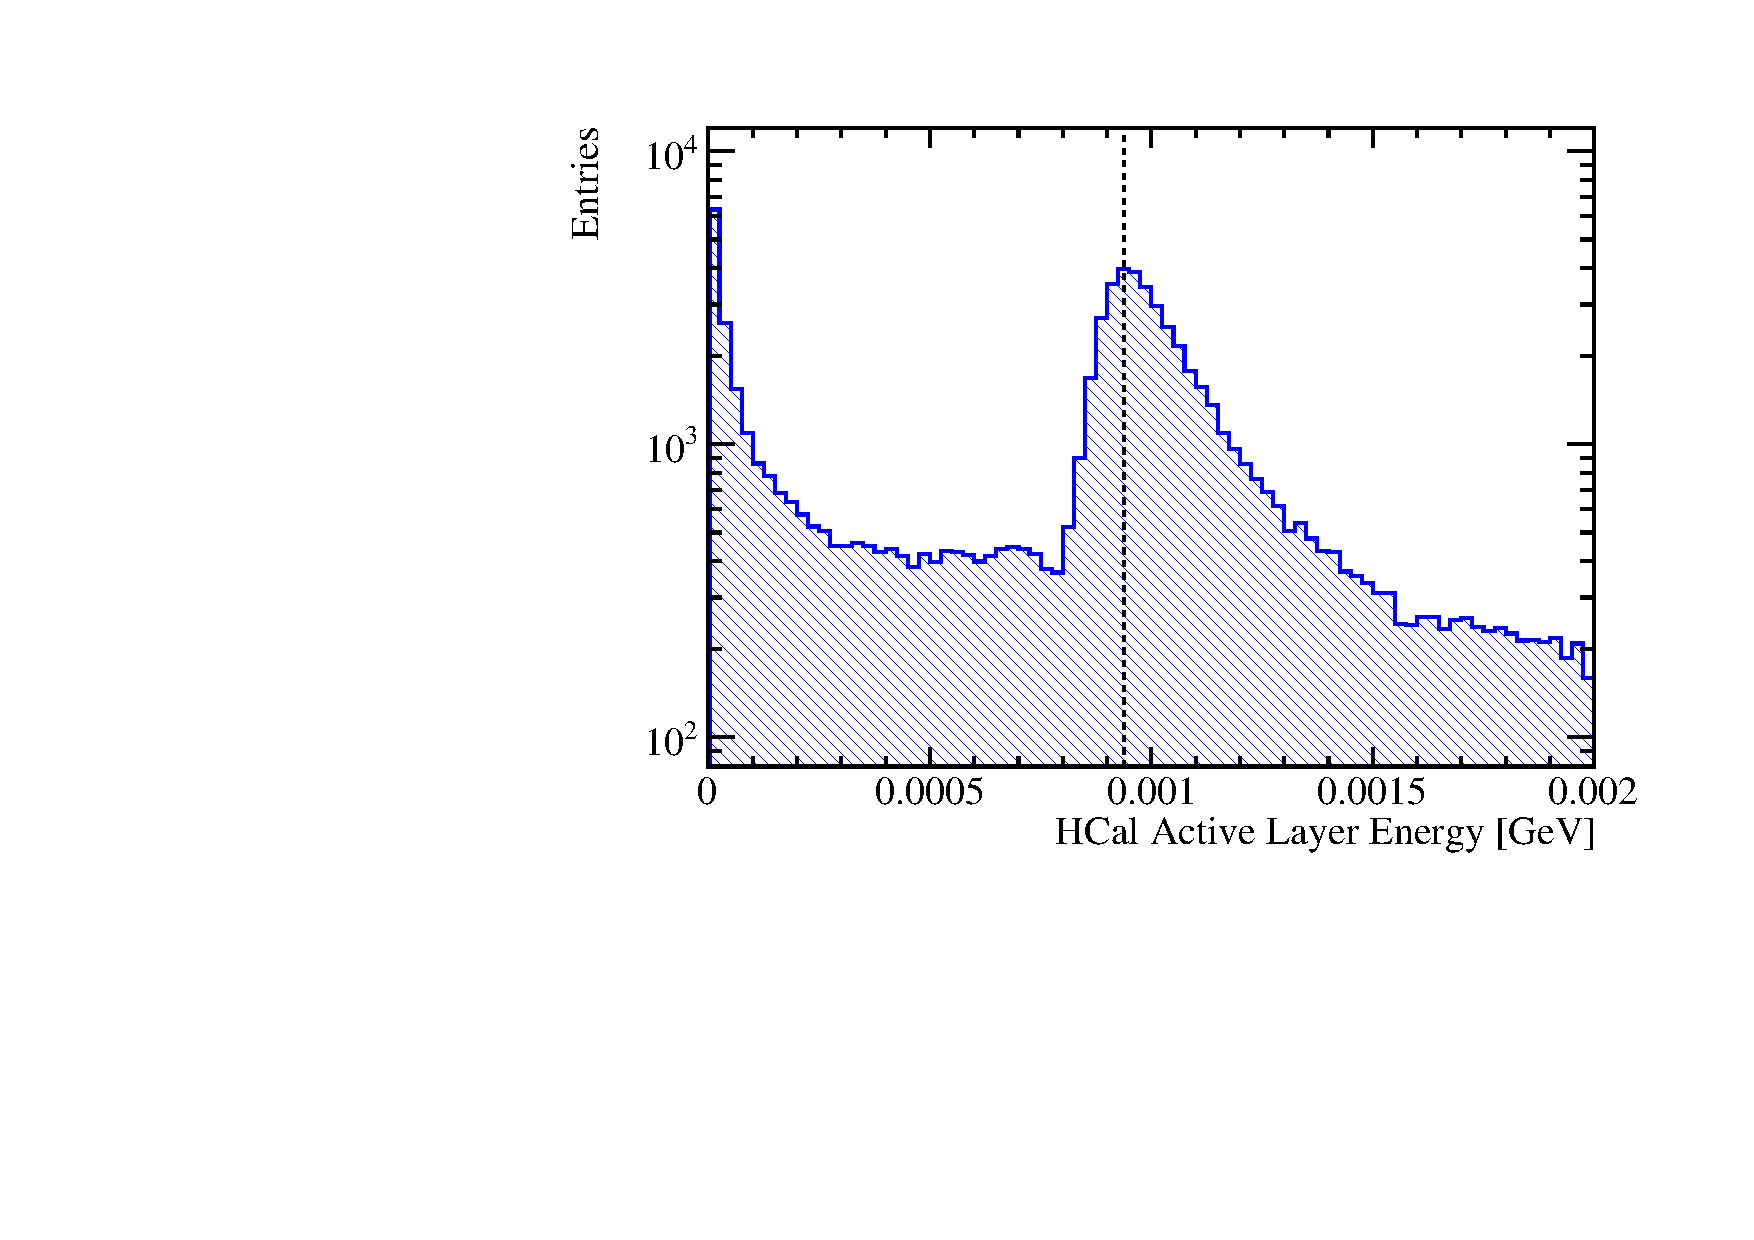
\includegraphics[width=0.5\textwidth]{EnergyEstimators/Plots/Calibration/MIPScale/Digitiser/MIPScaleDigitiserHCalOther.pdf}}
\caption[The active layer calorimeter cell energy distributions for various sub-detectors for 10 GeV $\mu^{-}$ events.]{The active layer calorimeter cell energy distributions for various sub-detectors for 10 GeV $\mu^{-}$ events.  The MIP peak is represented by the black dotted line.}
\label{fig:digitisermip}
\end{figure}

In the digitiser processor a single value for the MIP peak was required for the HCal and that was taken as the MIP peak position for the HCal Barrel.  The MIP peaks were separately calculated for the HCal EndCap and Ring for the purposes of the HCal Ring digitisation described in section \ref{sec:hcalringdigi}.  The realistic digitisation features present in the simulation of the ECal and HCal were not present for the muon chamber digitisation and so no MIP peak setting for that digitisation stage was required.

A similar procedure was employed for calculation of the MIP peak in PandoraPFA.  One important difference was the distribution used for setting the MIP scale in PandoraPFA is the distribution of calorimeter cell energies, i.e. the energy in the active and absorber layers of a cell, and not just the active layer energies.  Examples of the distributions used to set the MIP scale in PandoraPFA can be found in figure \ref{fig:pandoramip}.  There are few populated low calorimeter cell energy bins due to cuts applied in the digitiser on the minimum active layer energy required to make a calorimeter hit.  The double peak structure in the ECal calorimeter hit energy distribution is present due to the doubling of the thickness of the ECal absorber material, from 2.1 mm to 4.2 mm tungsten, in the ILD detector model, which occurs for the back the first 10 layers of the 30 layer ECal.  Two differences between the MIP scale setting in the digitiser and PandoraPFA worthy of note are that for the PandoraPFA MIP scale setting the HCal sub-detectors, the Barrel, EndCal and Ring, are all combined into a single cell energy distribution and PandoraPFA requires the MIP scale to be set in the muon chamber, which required a muon chamber cell energy distribution to be created.  

\begin{figure}
\subfloat[ECal.]{\label{fig:pandoramipecal}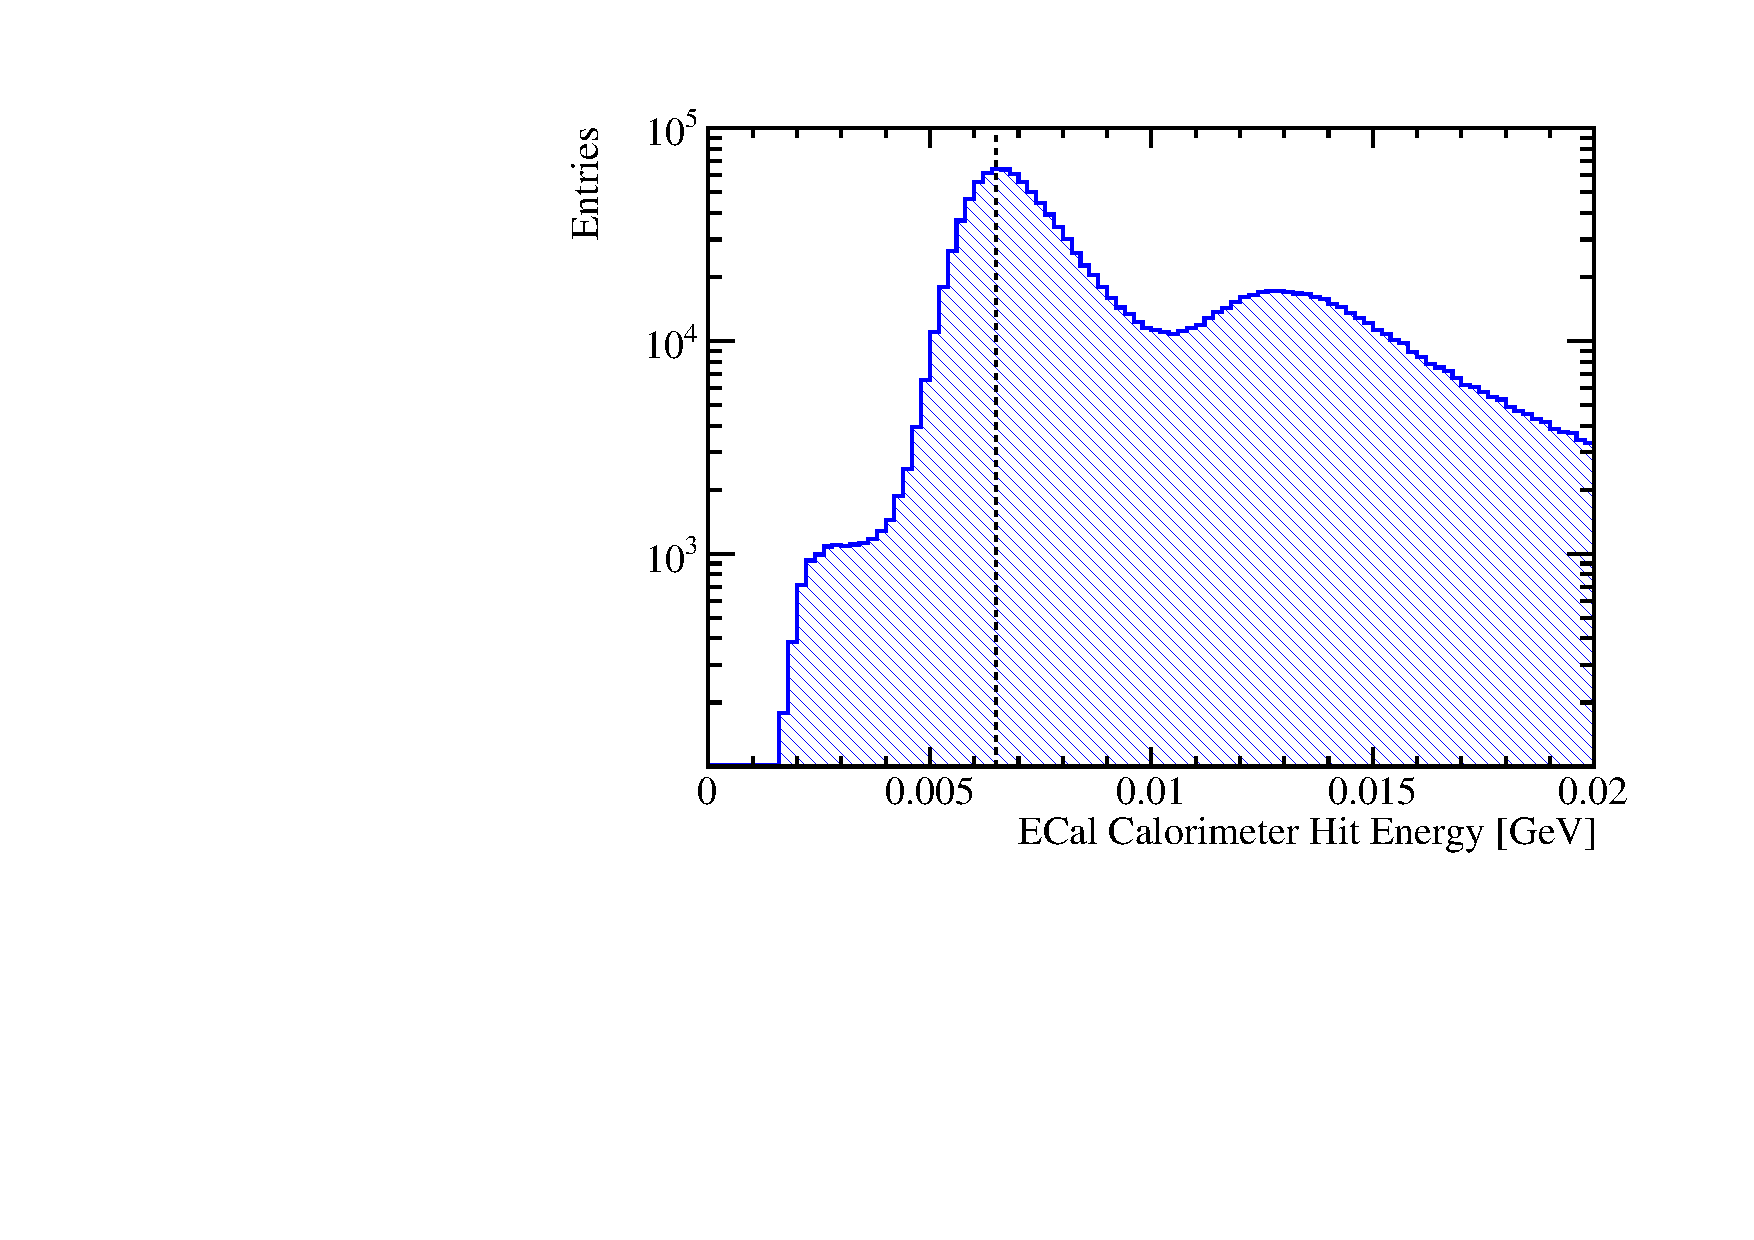
\includegraphics[width=0.5\textwidth]{EnergyEstimators/Plots/Calibration/MIPScale/PandoraPFA/MIPScalePandoraPFAECal.pdf}}
\subfloat[HCal.]{\label{fig:pandoramiphcal}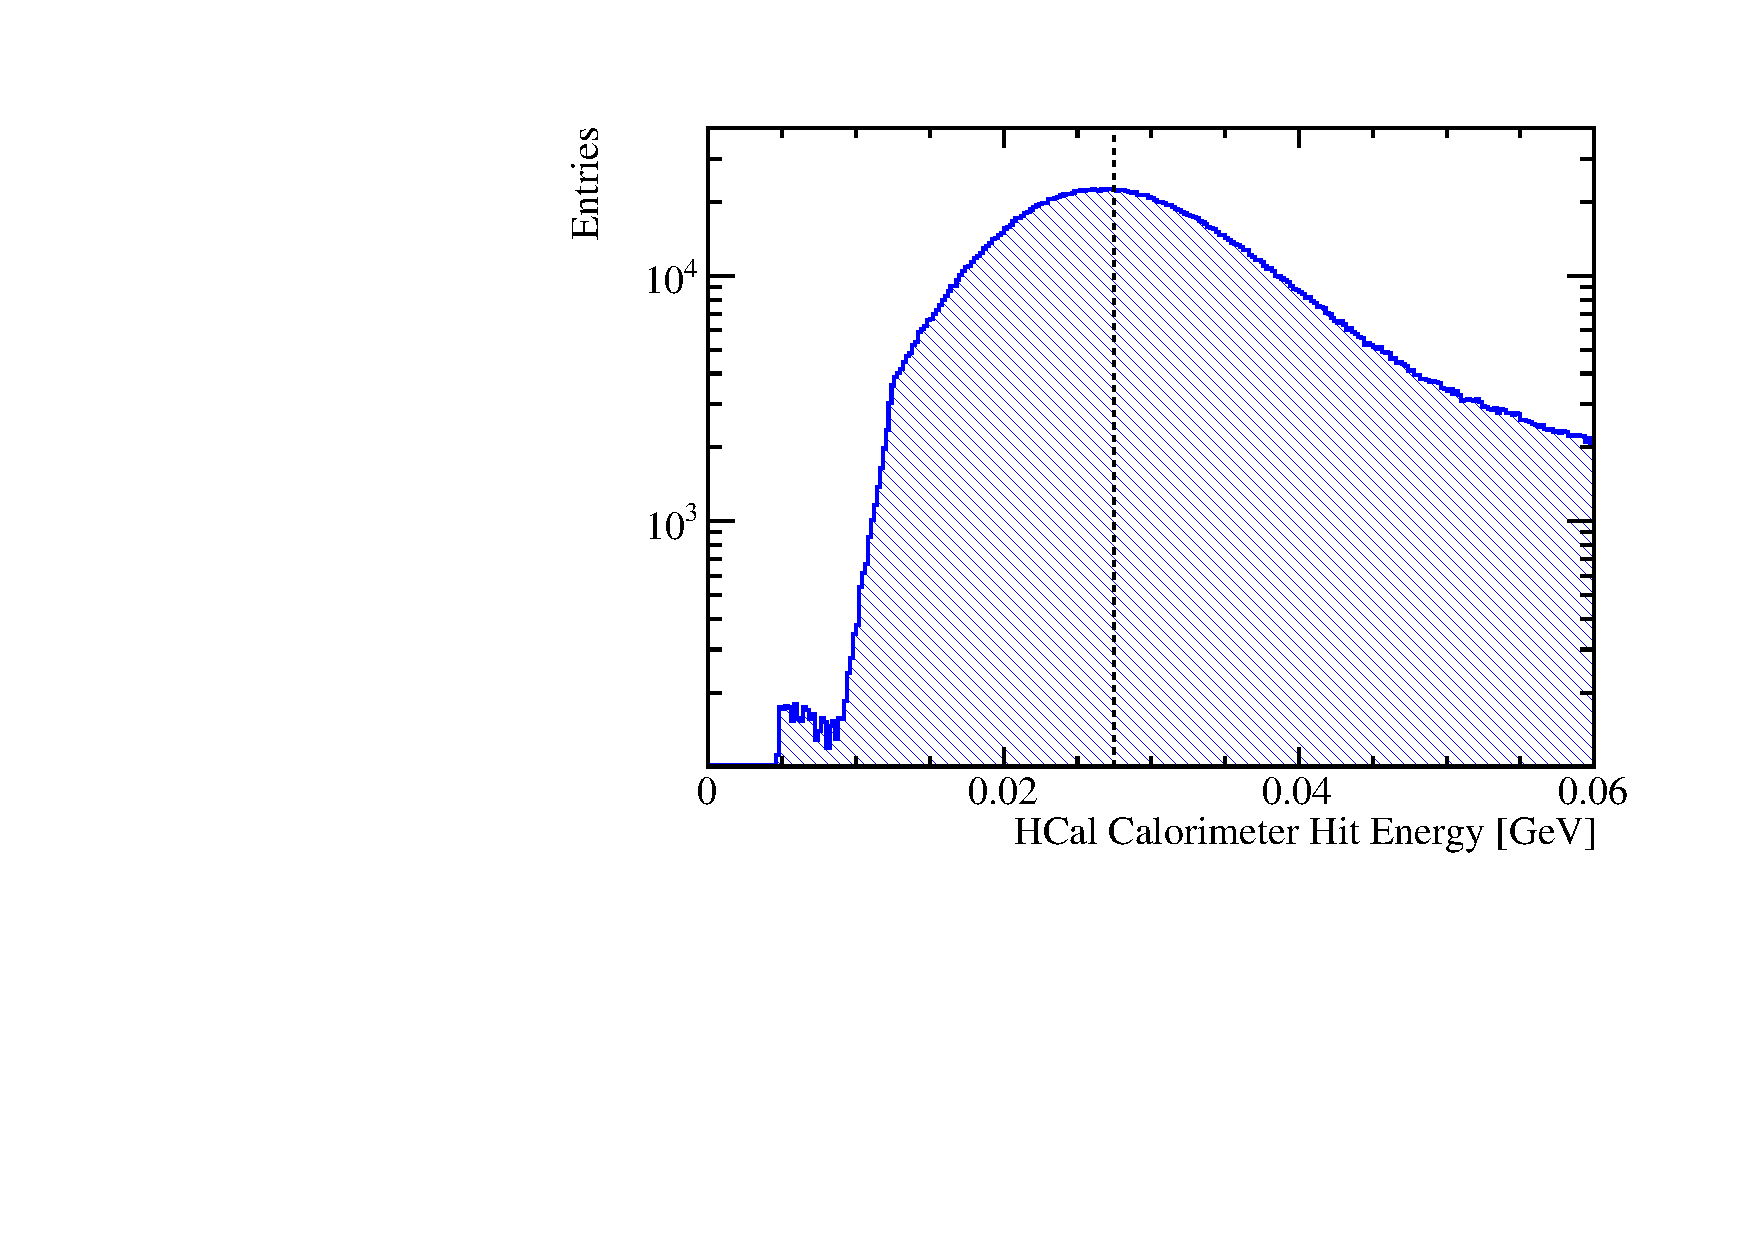
\includegraphics[width=0.5\textwidth]{EnergyEstimators/Plots/Calibration/MIPScale/PandoraPFA/MIPScalePandoraPFAHCal.pdf}} \\
\subfloat[Muon Chamber.]{\label{fig:pandoramipmuon}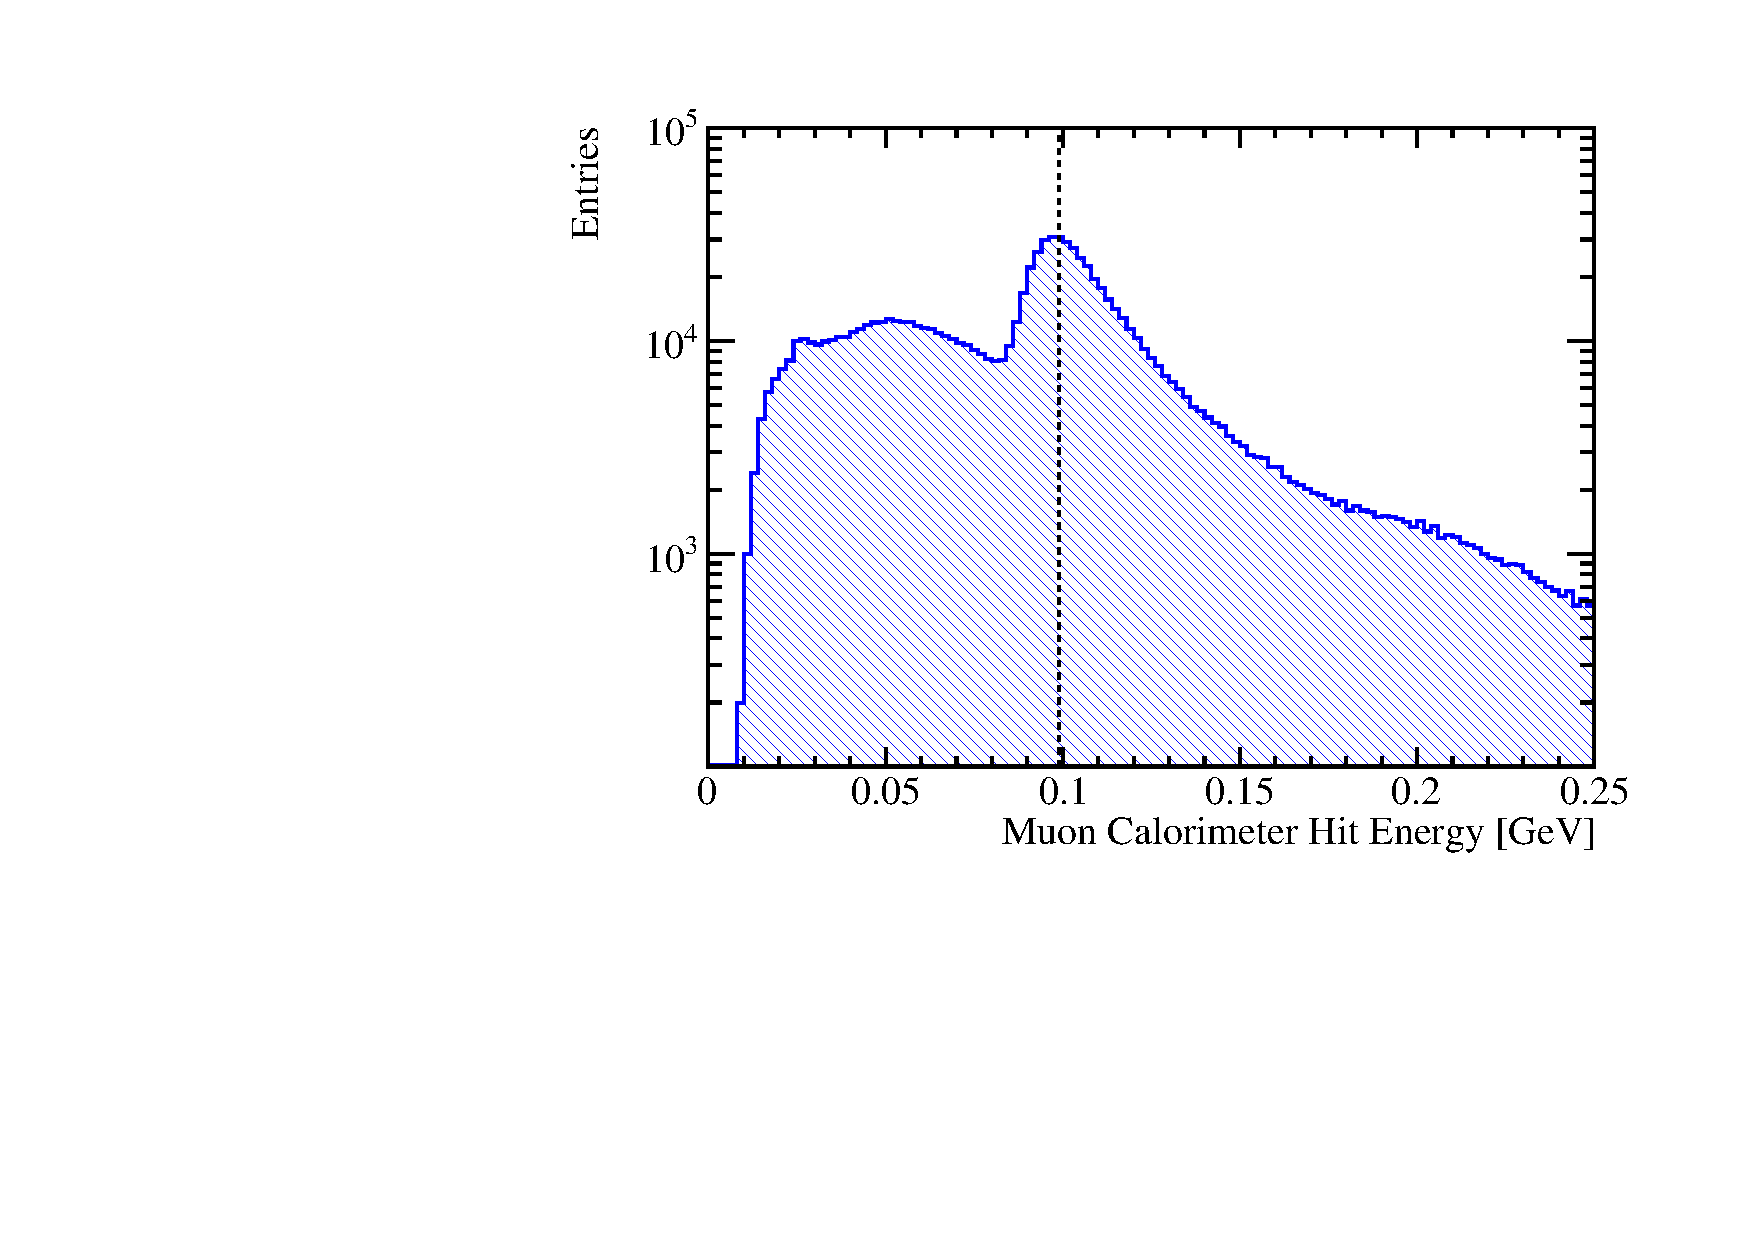
\includegraphics[width=0.5\textwidth]{EnergyEstimators/Plots/Calibration/MIPScale/PandoraPFA/MIPScalePandoraPFAMuon.pdf}}
\caption[The calorimeter cell energy distributions for various sub-detectors for 10 GeV $\mu^{-}$ events.]{The calorimeter cell energy distributions for various sub-detectors for 10 GeV $\mu^{-}$ events.  The MIP peak is represented by the black dotted line.}
\label{fig:pandoramip}
\end{figure}

%========================================================================================

\subsection{Electromagnetic and hadronic scale setting}
The electromagnetic and hadronic scales have to be independently set in the simulation to account for the different mechanisms governing the propagation of electromagnetic and hadronic showers.  As referenced earlier, one crucial difference the setting of these scales accounts for is the invisible energy component of hadronic showers, however, in this simulation it also accounts for the effect of energy loss due to the threshold cuts that are applied in the reconstruction.  The setting of the scales involves tuning four parameters in PandoraPFA, which correspond to the scaling factors that are applied to PFO energies arising from electromagnetic and hadronic showering particles in the ECal and HCal.  

%========================================================================================

\subsubsection{Electromagnetic scale setting}
\label{sec:emscalesetting}
The electromagnetic scale in the ECal, $\beta^{EM}_{ECal}$, is set in the detector using $\gamma$ events at $E_{MC} = 10$ GeV.  $\gamma$ events are ideal for the setting of the electromagnetic scale as they procedure electromagnetic showers and are primarily confined to the ECal at the energy considered as was shown in figure \ref{fig:ecaldigiphotonsplit}.  

Cuts are applied to ensure that only events where the bulk of the energy is deposited within the ECal are applied.  The cuts require a single $\gamma$ be reconstructed, excluding conversions, and that less than 1\% of the reconstructed energy is outside the ECal.  The impact of these cuts on the electromagnetic energy measured in the ECal for these 10 GeV $\gamma$ events is shown in figure \ref{fig:ecalemscaleselection}.

\begin{figure}
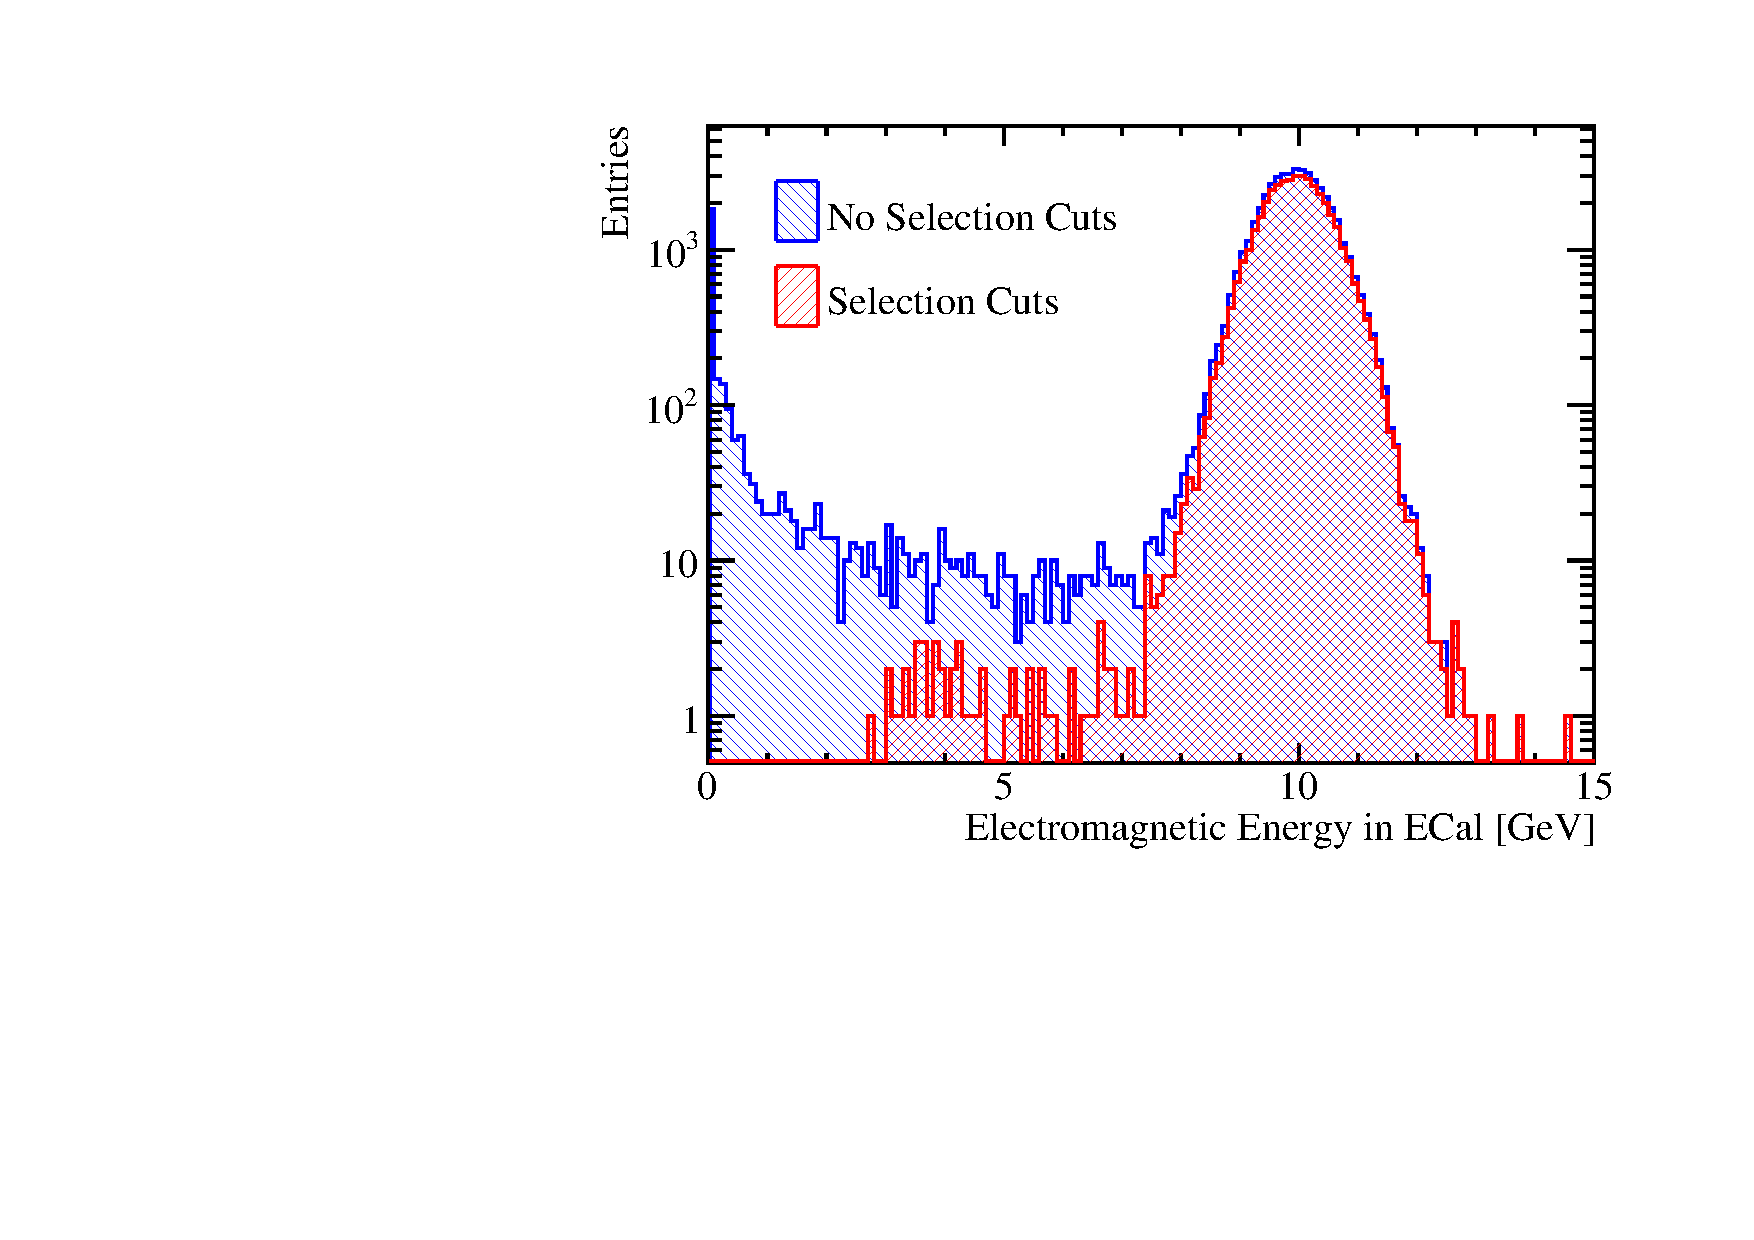
\includegraphics[width=0.5\textwidth]{EnergyEstimators/Plots/Calibration/EMScaleSetting/EMScaleECalSelection.pdf}
\caption[Sum of the electromagnetic energy measured in the ECal for 10 GeV $\gamma$ events with and without the selection cuts.]{Sum of the electromagnetic energy measured in the ECal for 10 GeV $\gamma$ events with and without the selection cuts.}
\label{fig:ecalemscaleselection}
\end{figure}

\begin{figure}
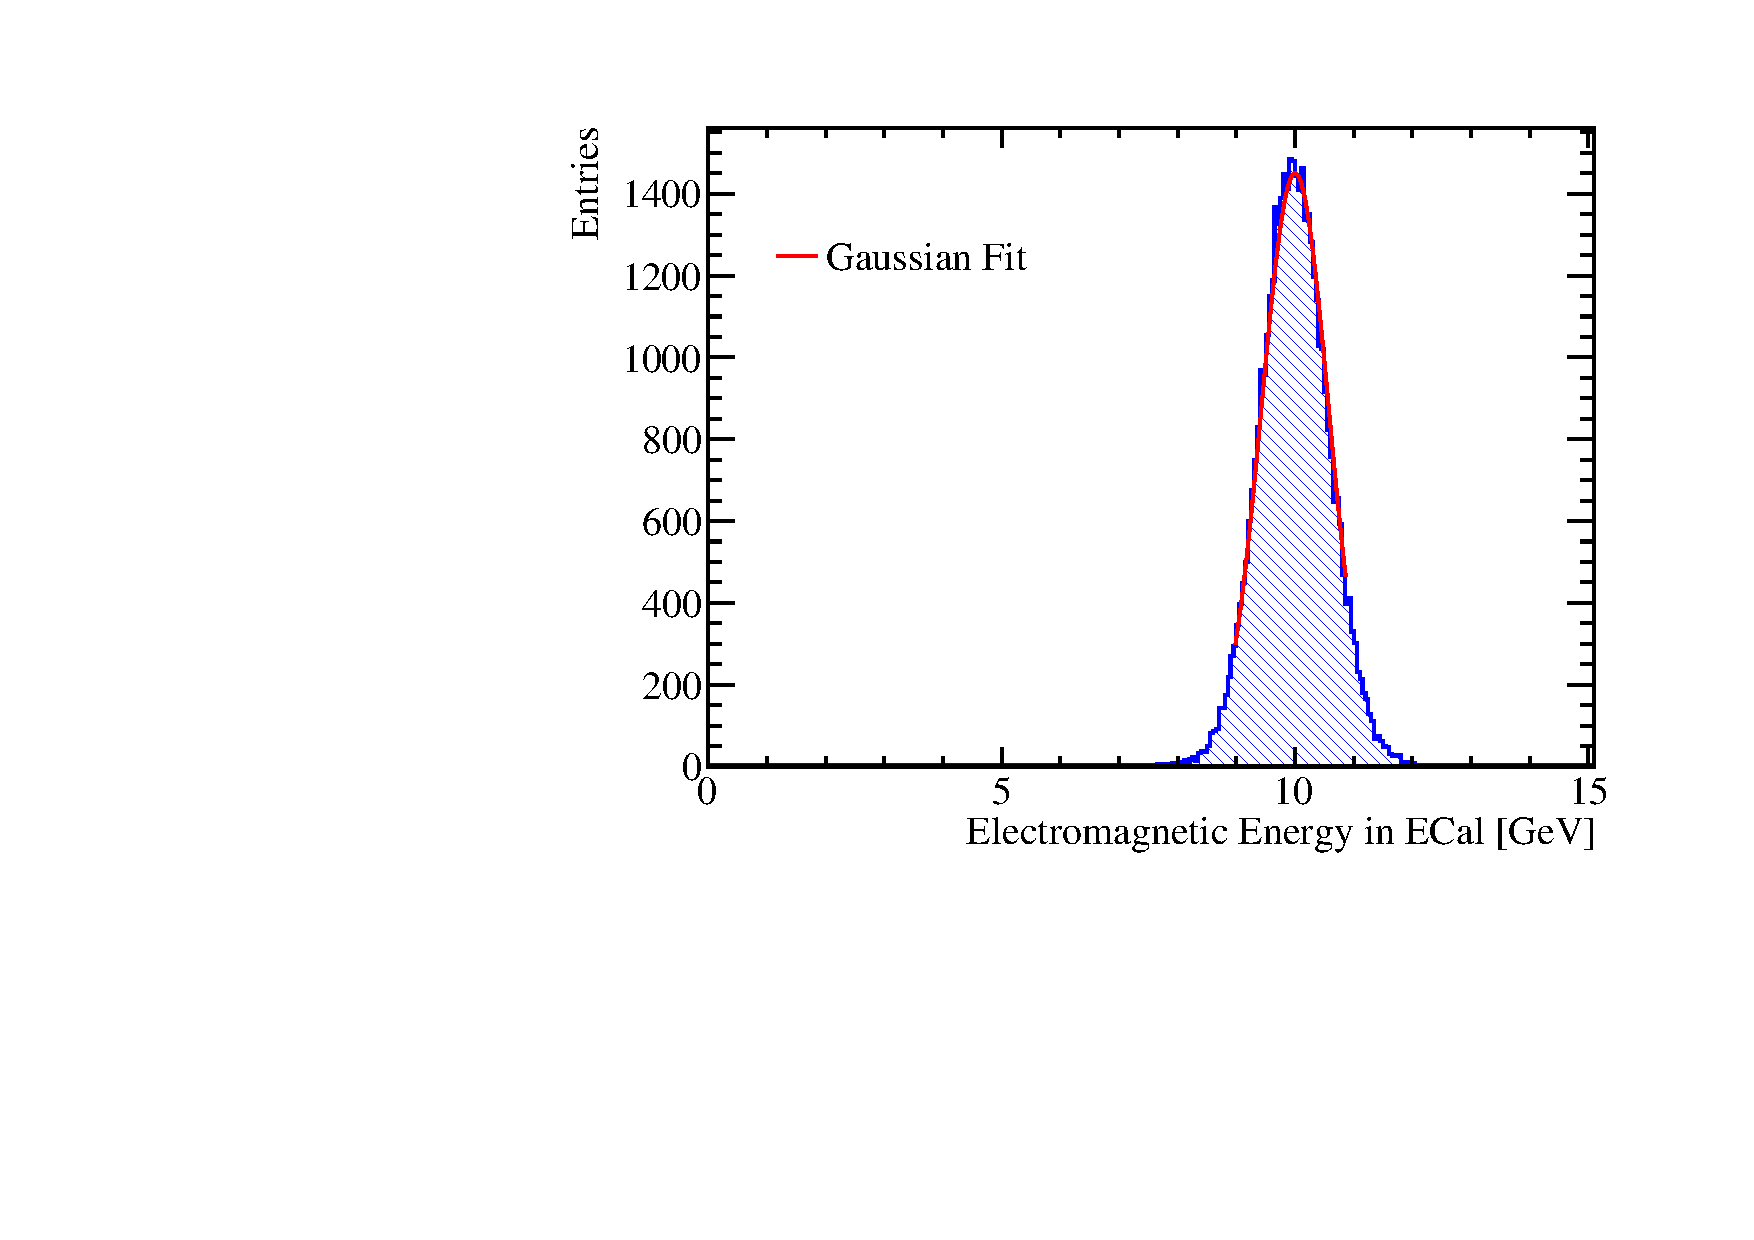
\includegraphics[width=0.5\textwidth]{EnergyEstimators/Plots/Calibration/EMScaleSetting/EMScaleSettingECalFit.pdf}
\caption[Gaussian fit to sum of the electromagnetic energy deposited in the ECal for 10 GeV $\gamma$ events with selection cuts.]{Gaussian fit to sum of the electromagnetic energy deposited in the ECal for 10 GeV $\gamma$ events with selection cuts.}
\label{fig:ecalemscalefit}
\end{figure}

The fitting procedure proceeds in a similar manor to that described in section \ref{sec:ecaldigi} whereby a trial calibration for the electromagnetic energy scale in the ECal, $\beta^{EM0}_{ECal}$, is assumed and the single $\gamma$ events simulated.  The distribution of the PFO electromagnetic energy in the ECal is produced and a Gaussian fit applied to the range of data with the smallest root mean square that contains at least 90 \% of the data.  The mean of this fit, $E_{\text{Fit}}$, is then used to scale $\beta^{EM0}_{ECal}$ in the following way

\begin{equation}
\beta^{EM0}_{ECal} \rightarrow \beta^{EM}_{ECal} = \beta^{EM0}_{ECal} \times \frac{E_{MC}}{E_{Fit}}
\end{equation}

An example distribution and fit used for calibration of the nominal ILD detector model can be found in figure \ref{fig:ecalemscalefit}.  The procedure is then repeated using the updated $\beta^{EM}_{ECal}$ until $E_{\text{Fit}}$ falls within a chosen tolerance, which in this case is that $|E_{\text{Fit}} - E_{\text{MC}}| < E_{\text{MC}} \times 0.5 \%$.  The binning for the fitted histogram is chosen such that the bin width is equal to the desired tolerance on $E_{\text{Fit}}$ e.g. $E_{\text{MC}} \times 0.5 \% = 0.05$ GeV.  This tolerance is tighter than that applied for the digitisation as it is the PFO energies that are used in downstream analyses and therefore require high precision. 
 
The electromagnetic scale in the HCal, $\beta^{EM}_{HCal}$, is chosen to be equal to the hadronic scale in the HCal, $\beta^{Had}_{HCal}$.  The details of the determination of $\beta^{Had}_{HCal}$ can be found in section \ref{sec:hadscalesetting}.  For ILC like energies, $\beta^{EM}_{HCal}$ is not a critical parameter in the reconstruction as photons are largely contained within the ECal meaning little to no electromagnetic energy is measured in the HCal.  

%========================================================================================

\subsubsection{Hadronic scale setting}
\label{sec:hadscalesetting}
$\beta^{Had}_{ECal}$ is important to detector performance as a non-negligible amount of hadronic energy is recorded in the ECal.  However, as the ECal contains $\approx 1 \lambda_{I}$, the hadronic scale in the ECal cannot be independently as it is unfeasible to create a large sample of 20 GeV $K^{0}_{L}$ events that are fully contained within it.  Therefore, the hadronic scale is set in the ECal and HCal simultaneously.  

Cuts applied to select $K^{0}_{L}$ that are appropriate to use for the hadronic scale calibration.  The last layer in which energy is deposited in the HCal must not occur in the back 10 \% of the HCal to ensure the event will not suffer from leakage.  A single neutral hadron must be reconstructed to veto events with reconstruction failures.  Finally, the total hadronic energy measured in ECal and HCal, $E^{Had}_{ECal} + E^{Had}_{HCal}$, must fall within 3 $\sigma$ of the desired hadronic energy distribution, $E^{Had}_{ECal} + E^{Had}_{HCal} = 20 \text {GeV} - m_{K^{0}_{L}} = E_{MC}$.  $\sigma$ is defined to be $55\% \times \sqrt{E} = 2.46 \text{GeV}$ for 20 GeV $K^{0}_{L}$.  This definition of sigma is the nominal energy resolution for neutral hadrons in the ILD HCal.  This cut ensures that when fitting the two dimensional distribution of hadronic energy measured in the ECal and HCal the outliers do not skew the fit.  These cuts are illustrated in in figure \ref{fig:hadscaleselection}.

\begin{figure}
\subfloat[]{\label{fig:hadscaleselectionnocuts}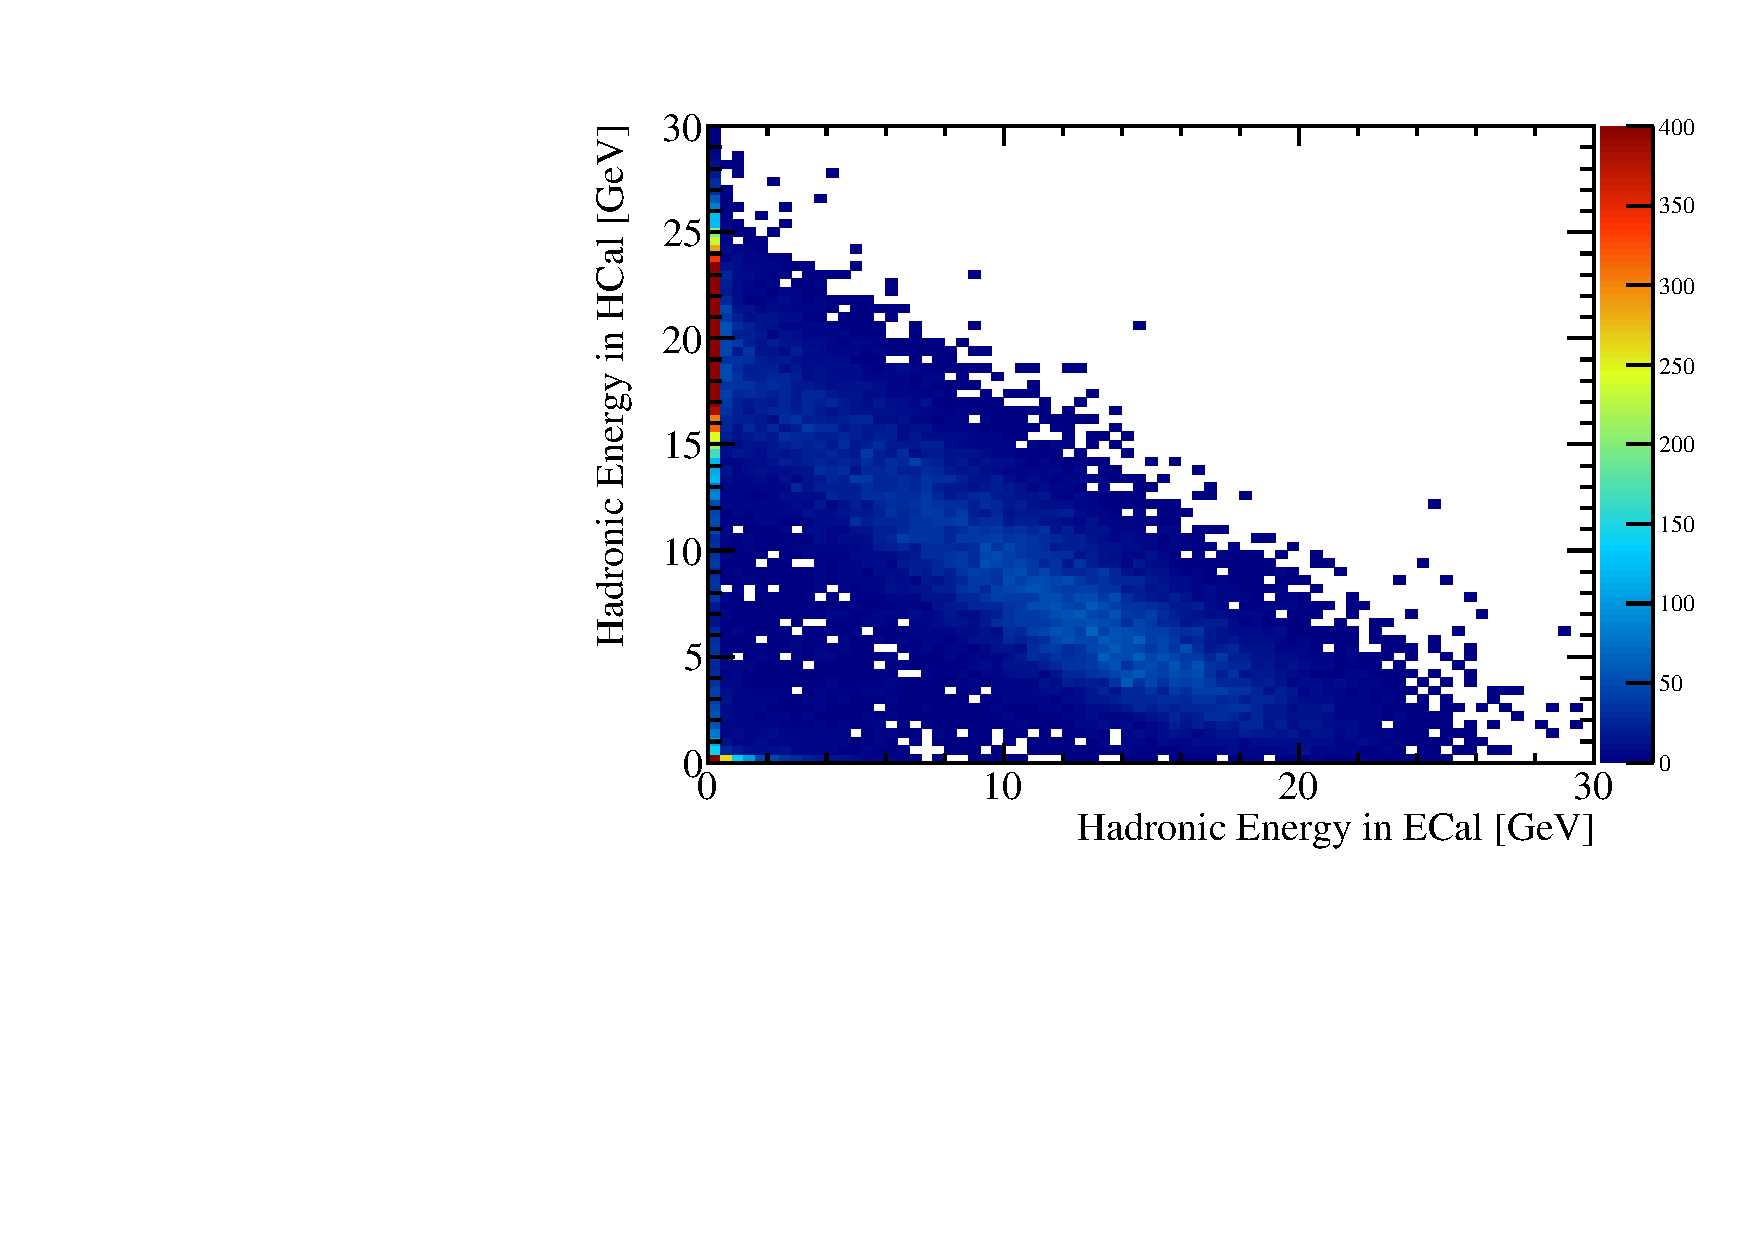
\includegraphics[width=0.5\textwidth]{EnergyEstimators/Plots/Calibration/HadScaleSetting/HadScaleECalHCalSelectionNoCuts.pdf}}
\subfloat[]{\label{fig:hadscaleselectioncuts}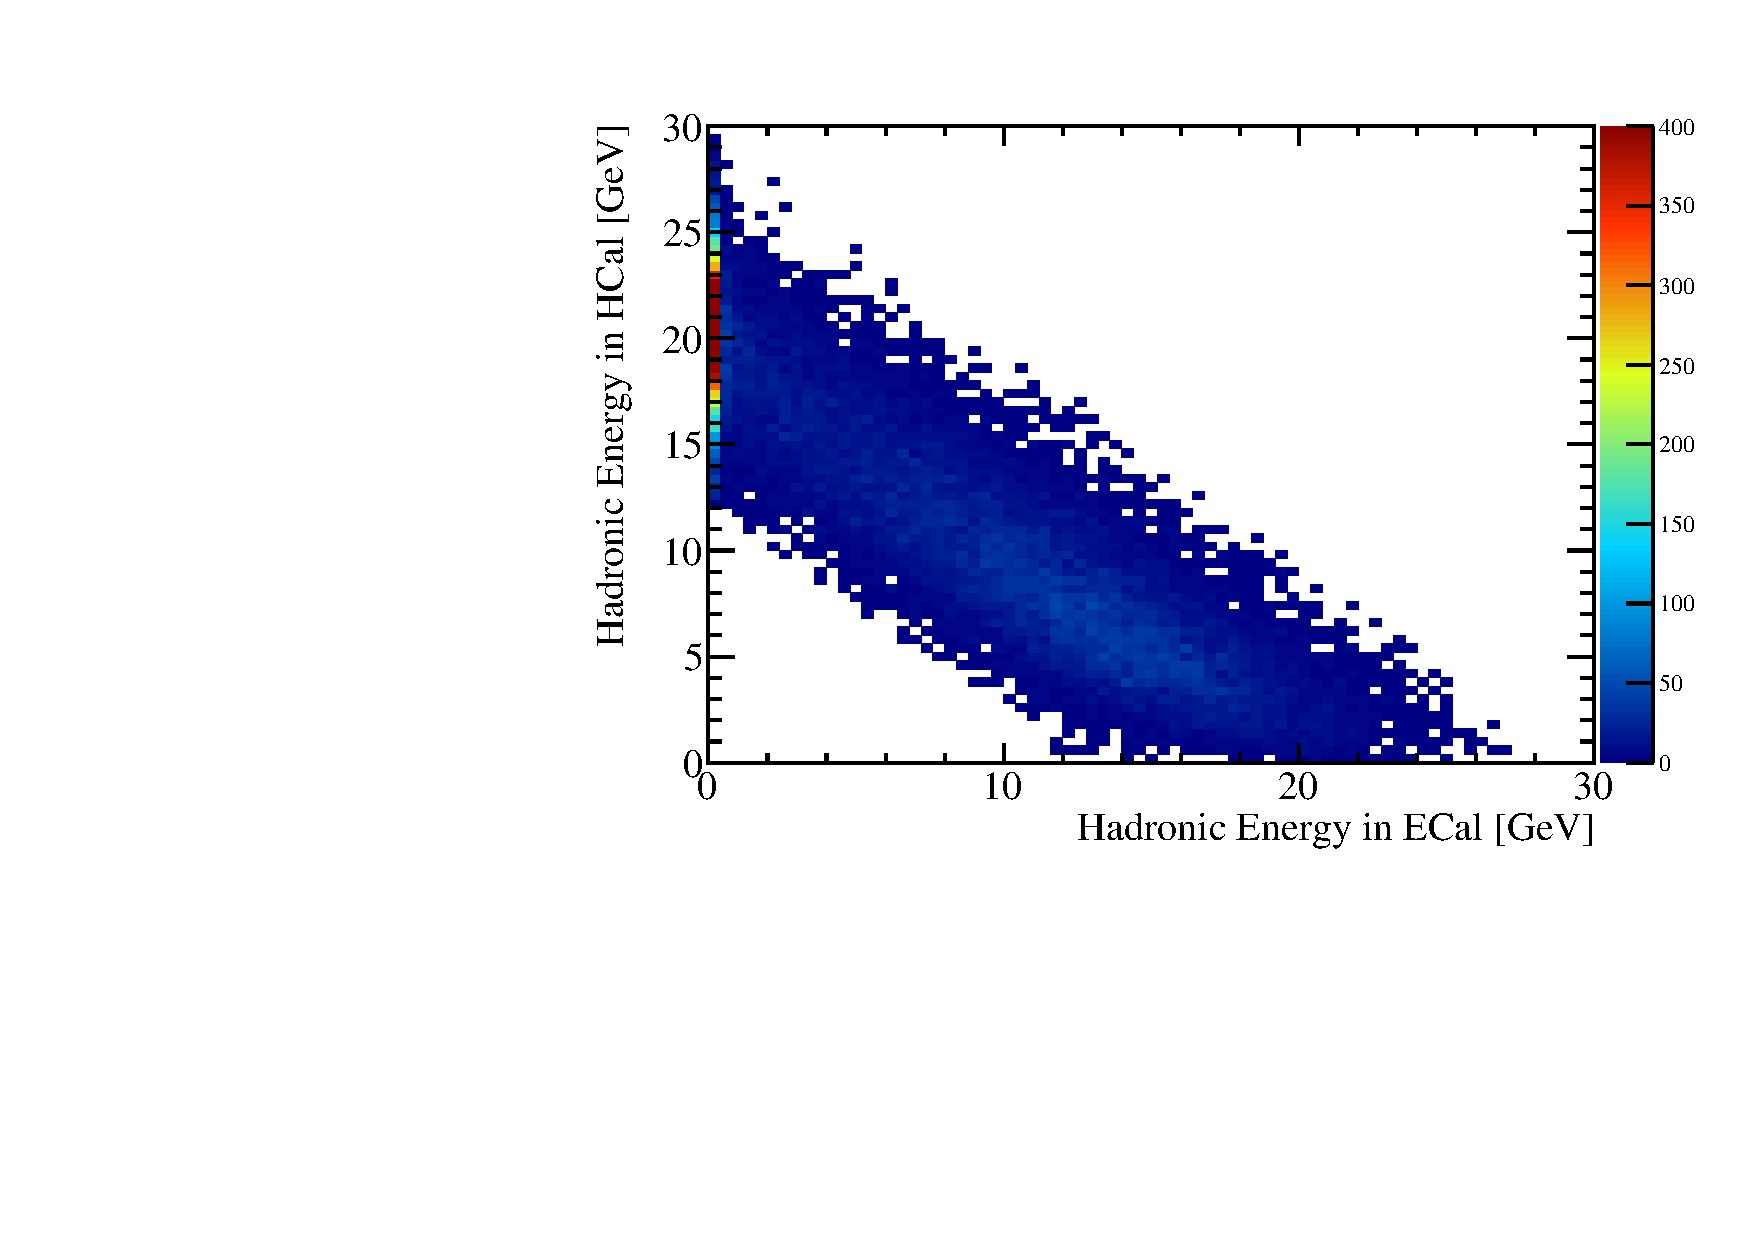
\includegraphics[width=0.5\textwidth]{EnergyEstimators/Plots/Calibration/HadScaleSetting/HadScaleECalHCalSelectionCuts.pdf}}
\caption[The distribution of hadronic energy measured in the ECal and HCal for 20 GeV $K^{0}_{L}$ events with and without selection cuts.]{The distribution of hadronic energy measured in the ECal and HCal for 20 GeV $K^{0}_{L}$ events \protect\subref{fig:hadscaleselectionnocuts} without selection cuts and \protect\subref{fig:hadscaleselectioncuts} with selection cuts.}
\label{fig:hadscaleselection}
\end{figure}

The calibration procedure is iterative and begins by assuming trial values, $\beta^{Had0}_{ECal}$ and $\beta^{Had0}_{ECal}$, for the hadronic scale calibration factors $\beta^{Had}_{ECal}$ and $\beta^{Had}_{ECal}$.  The 20 GeV $K^{0}_{L}$ events are then simulated and reconstructed.  Following this a linear fit to the distribution of $E^{Had}_{ECal}$ against $E^{Had}_{HCal}$ for 20 GeV $K^{0}_{L}$ events passing the selection cuts is applied.  The fit is performed by minimising $\chi^{2}$, which is defined as

\begin{equation}
\chi^{2}(\delta^{Had}_{ECal}, \delta^{Had}_{HCal}) = \sum_{i} \frac{x_{i}}{\sigma_{x_{i}}}
\end{equation}

where $x_{i}$ is the perpendicular distance from $E^{Had}_{ECal}$ and $E^{Had}_{HCal}$ for event $i$ to the line $E^{Had}_{HCal} = \delta^{Had}_{HCal} - E^{Had}_{ECal} \frac{\delta^{Had}_{HCal}}{\delta^{Had}_{ECal}}$.   The definition of $x_{i}$ is given in equation \ref{equ:xicalc}, but best illustrated by considering figure \ref{fig:hadscalechi2calc}.  $\sigma_{x_{i}}$ is the uncertainty on $x_{i}$, which is calculated by propagating the uncertainties on $E^{Had}_{ECal}$ and $E^{Had}_{HCal}$, which are assumed to be $\sigma_{E^{Had}_{E/HCal}} = 55\% \times \sqrt{E^{Had}_{E/HCal}}$, into the expression for $x_{i}$.  The result of this propagation of errors is given in equation \ref{equ:sigmaxicalc}.  The sum runs over all events, $i$, passing the selection cuts.  

\begin{figure}
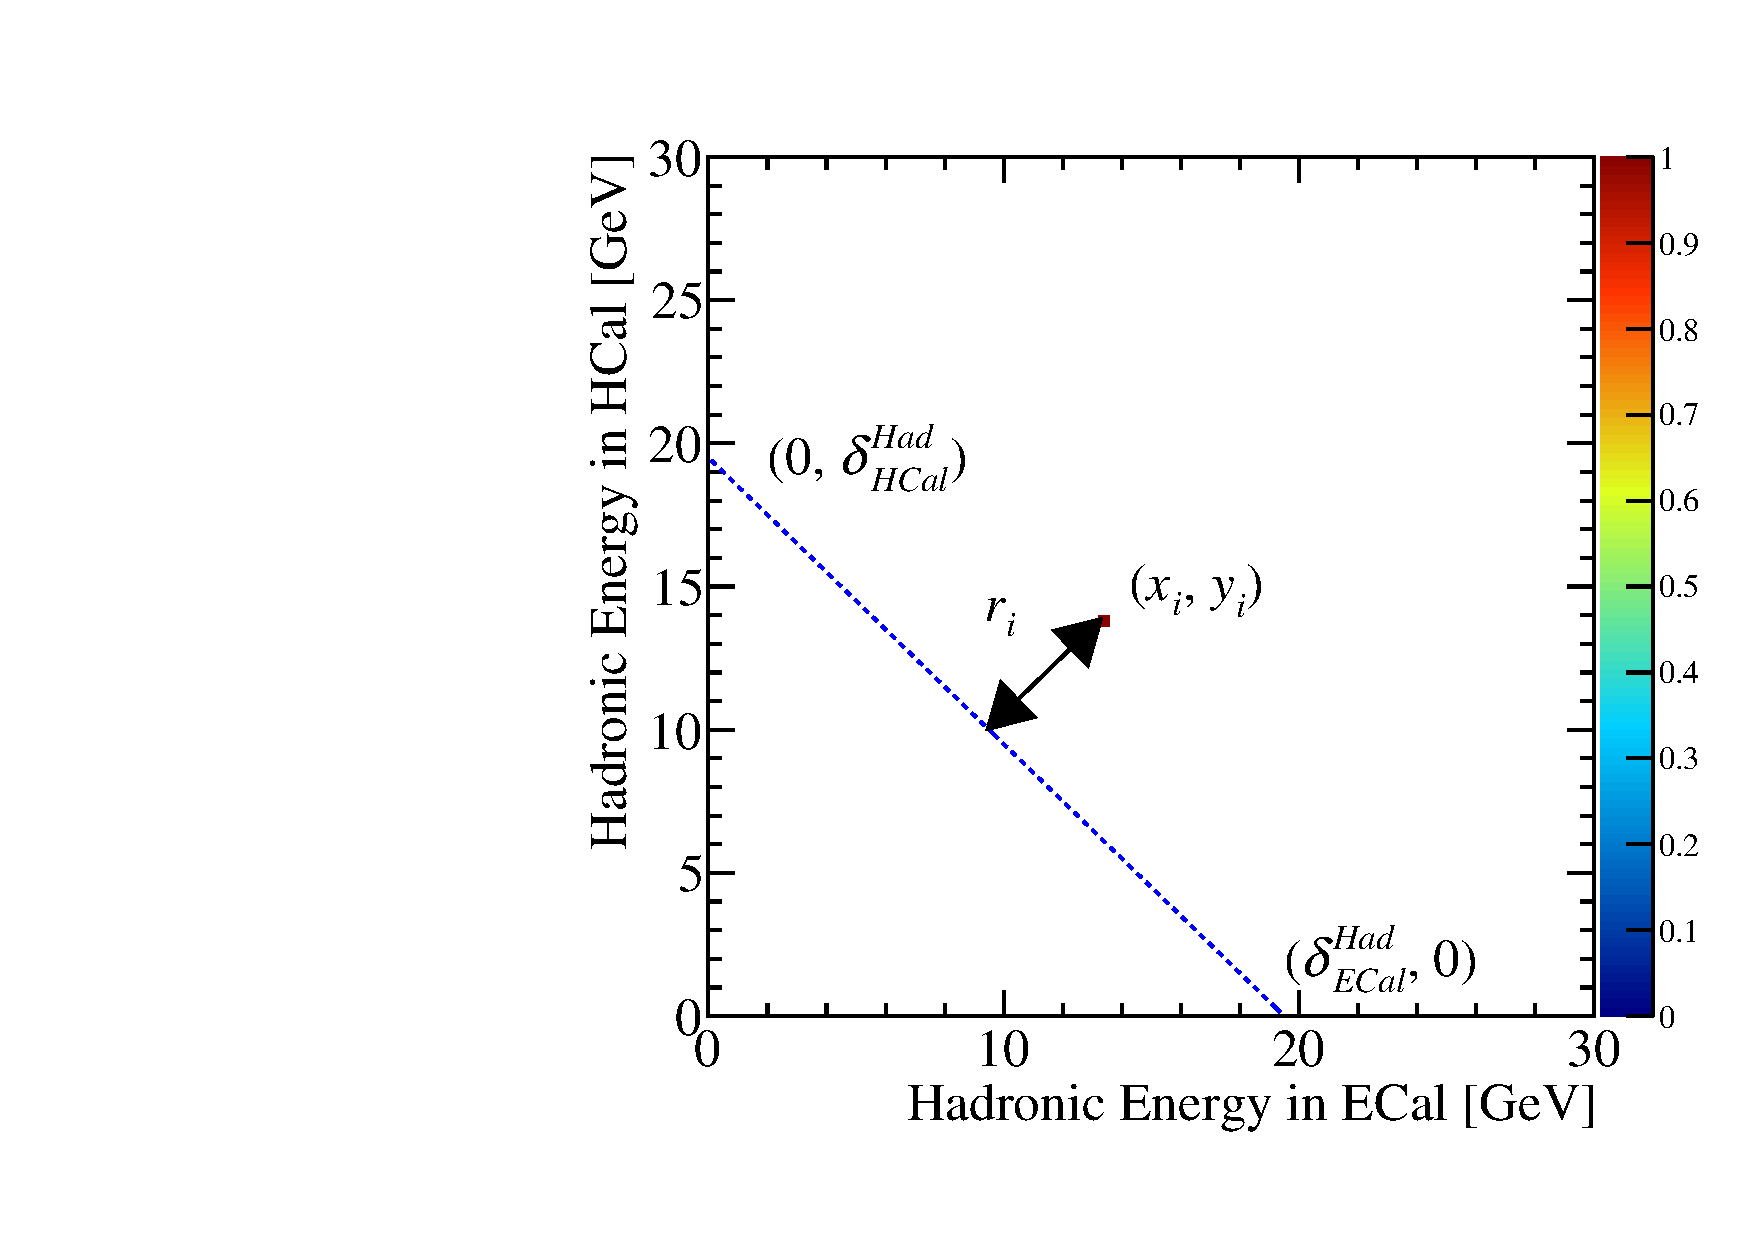
\includegraphics[width=0.5\textwidth]{EnergyEstimators/Plots/Calibration/HadScaleSetting/HadScaleECalHCalSelectionExample.pdf}
\caption[An example showing the definition of $x_{i}$, the variable used for the calculation of $\chi^{2}(\delta^{Had}_{ECal}, \delta^{Had}_{HCal})$ for the setting of the hadronic energy scale.]{An example showing the definition of $x_{i}$, the variable used for the calculation of $\chi^{2}$ for the setting of the hadronic energy scale.  For an event that has been measured with hadronic energy $E^{Had}_{ECal}$ in the ECal and $E^{Had}_{HCal}$ in the HCal, the geometric interpretation of $x_{i}$ is shown.  The blue dotted line is defined as $E^{Had}_{HCal} = \delta^{Had}_{HCal} - E^{Had}_{ECal} \frac{\delta^{Had}_{HCal}}{\delta^{Had}_{ECal}}$.}
\label{fig:hadscalechi2calc}
\end{figure}

\begin{equation}
x_{i} = \frac{E^{Had}_{HCal} \delta^{Had}_{ECal} + E^{Had}_{ECal} \delta^{Had}_{HCal} - \delta^{Had}_{ECal} \delta^{Had}_{HCal}}{\sqrt{(\delta^{Had}_{ECal})^{2} + (\delta^{Had}_{HCal})^{2}}}
\label{equ:xicalc}
\end{equation}

\begin{equation}
\sigma_{i} = \frac{(\sigma_{E^{Had}_{HCal}}  \delta^{Had}_{ECal})^{2} + (\sigma_{E^{Had}_{ECal}} \delta^{Had}_{HCal})^{2}}{\sqrt{(\delta^{Had}_{ECal})^{2} + (\delta^{Had}_{HCal})^{2}}}
\label{equ:sigmaxicalc}
\end{equation}

The minimisation steps across a range of $\delta^{Had}_{ECal}$ and $\delta^{Had}_{HCal}$ centred about the ideal value of $20 \text { GeV} - m_{K^{0}_{L}}$ in search for the minimum $\chi^{2}$.  Once the minima in $\chi^{2}$ is found the trial calibration factors $\beta^{Had0}_{ECal}$ and $\beta^{Had0}_{ECal}$ are rescaled to correct for any deviation from the desired fit as follows

\begin{equation}
\beta^{Had0}_{ECal} \rightarrow \beta^{Had}_{ECal} = \beta^{Had0}_{ECal} \times \frac{E_{MC}}{\Delta^{Had}_{ECal}} \\
\beta^{Had0}_{HCal} \rightarrow \beta^{Had}_{HCal} = \beta^{Had0}_{HCal} \times \frac{E_{MC}}{\Delta^{Had}_{HCal}}
\end{equation}

where $\Delta^{Had}_{ECal}$ and $\Delta^{Had}_{ECal}$ are the values of $\delta^{Had}_{ECal}$ and $\delta^{Had}_{ECal}$ giving the minimum $\chi^{2}$.  The step sizes used for minimising $\chi^{2}$ with respect to $\delta^{Had}_{ECal}$ and $\delta^{Had}_{ECal}$ is chosen such that a single step corresponds to the target final tolerance on $\delta^{Had}$ i.e. $|\delta^{Had}_{E/HCal} - E_{\text{MC}}| < E_{\text{MC}} \times 0.5 \% \approx 0.1 \text{GeV}$.  

This procedure is then repeated until $\Delta^{Had}_{ECal}$ and $\Delta^{Had}_{ECal}$ both fall within a given tolerance, which in this case it taken to be $|\Delta^{Had}_{E/HCal} - E_{\text{MC}}| < E_{\text{MC}} \times 0.5 \% \approx 0.1 \text{GeV}$

%========================================================================================



%========================================================================================



\iffalse

\begin{figure}
  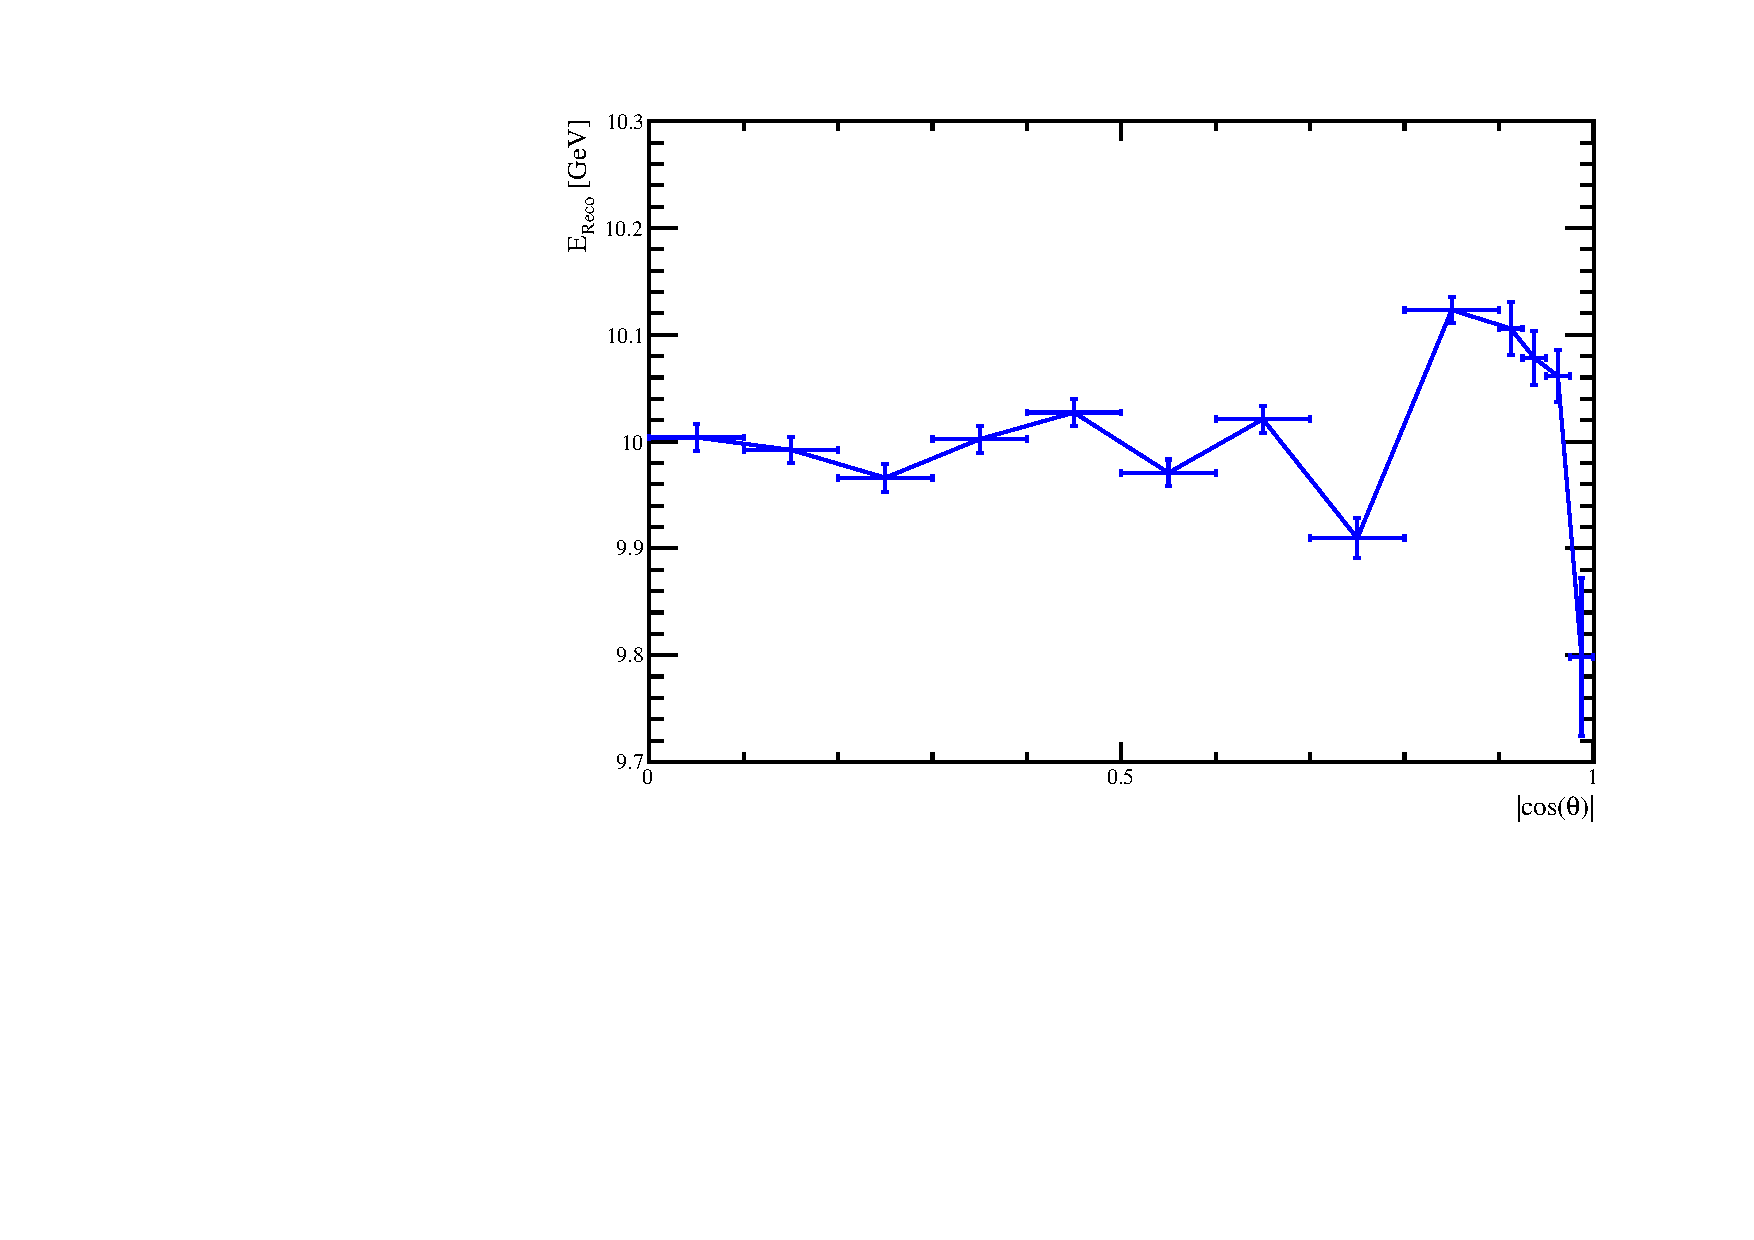
\includegraphics[width=0.5\textwidth]{EnergyEstimators/Plots/Calibration/Validation/AngularDistributionPhotonPlot.pdf}
  \caption[Mean reconstructed photon energy as a function of the polar angle of the photon.]{Mean reconstructed photon energy as a function of the polar angle of the photon.}
  \label{engest:fig:photonangle}
\end{figure}

\begin{figure}
  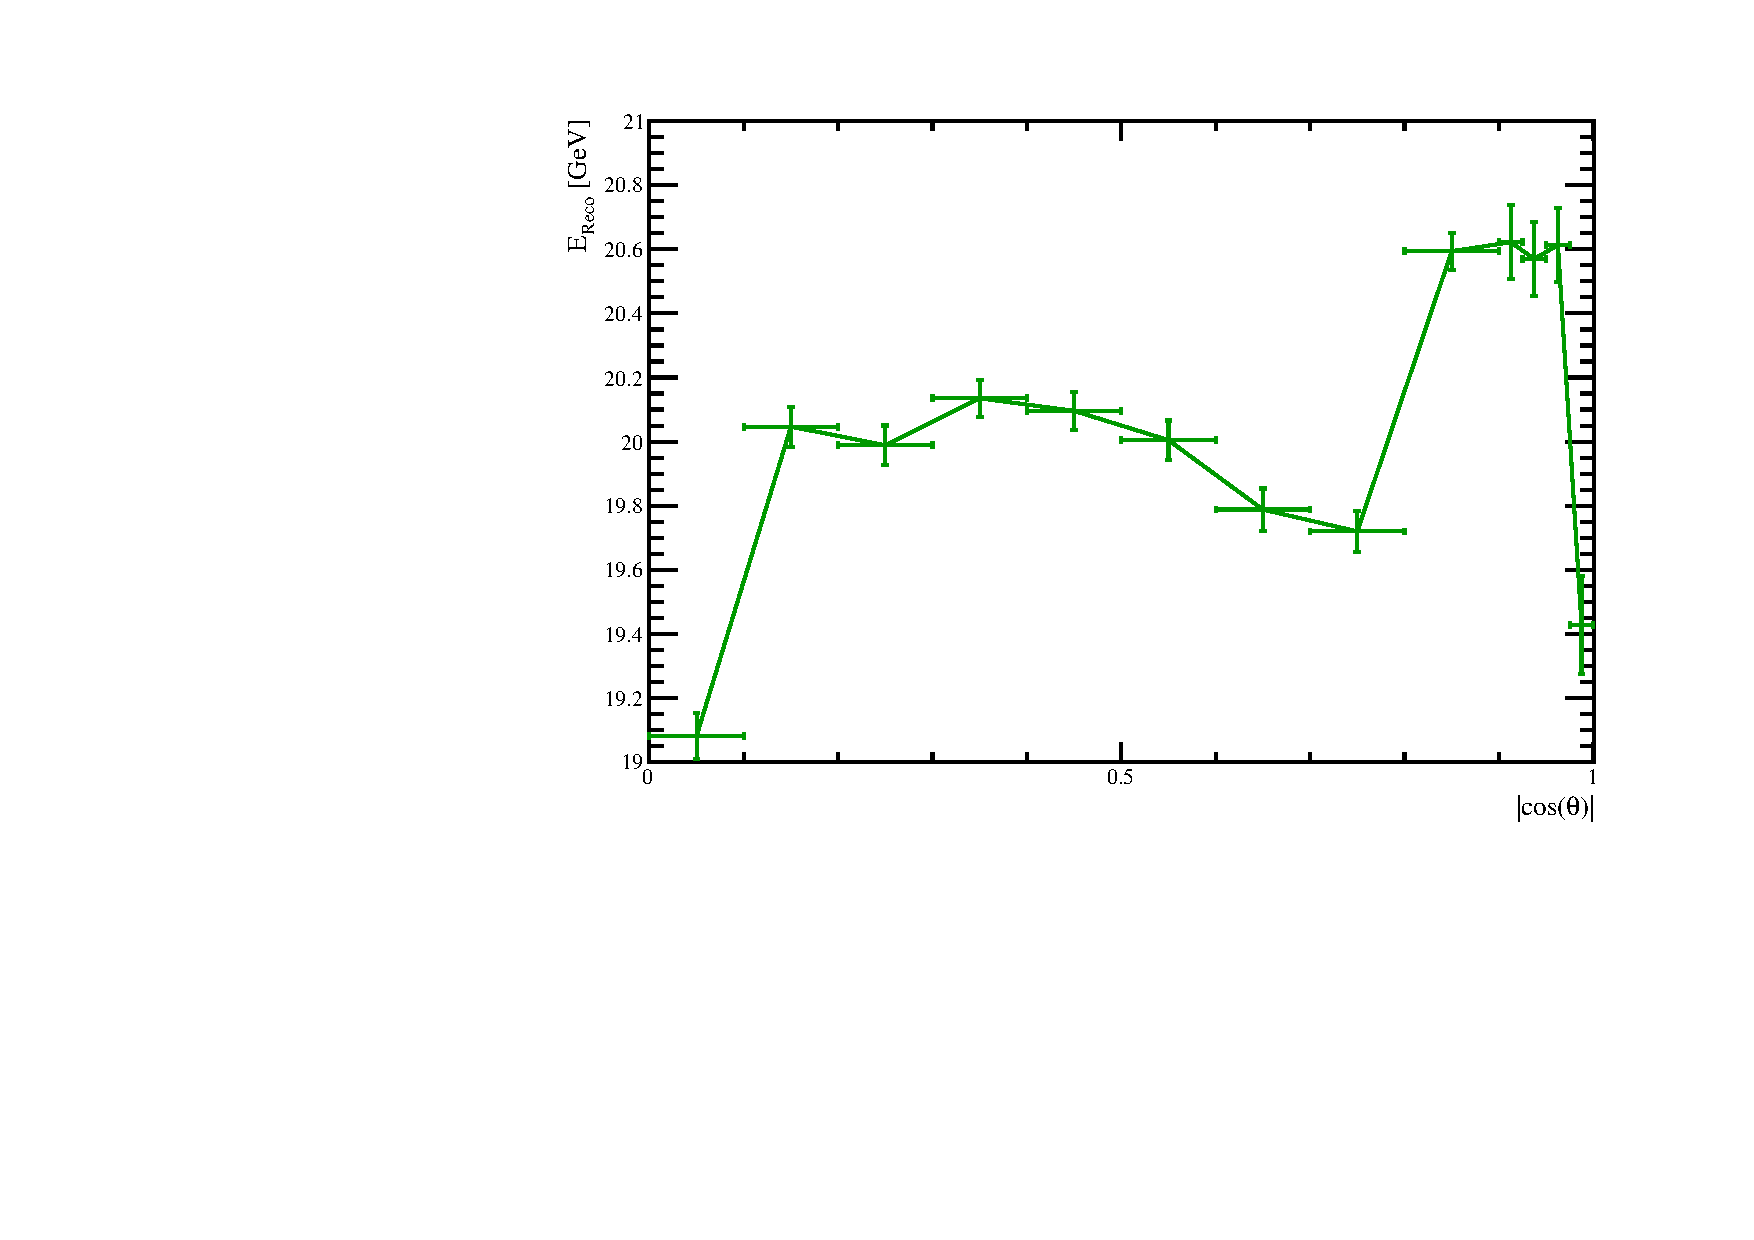
\includegraphics[width=0.5\textwidth]{EnergyEstimators/Plots/Calibration/Validation/AngularDistributionKaon0LPlot.pdf}  \caption[Mean reconstructed kaon0L energy as a function of the polar angle of the kaon0L.]{Mean reconstructed kaon0L energy as a function of the polar angle of the kaon0L.}
    \label{engest:fig:photonangle}
    \end{figure}
    
Validation 
/Users/stevengreen/Thesis/EnergyEstimators/Plots/Calibration/Validation
207:Validation stevengreen
AngularDistributionKaon0LPlot.pdf AngularDistributionPhotonPlot.pdf

SoftComp
/Users/stevengreen/Thesis/EnergyEstimators/Plots/SoftComp/DrawWeights.C /Users/stevengreen/Thesis/EnergyEstimators/Plots/SoftComp/MakePlots.C /Users/stevengreen/Thesis/EnergyEstimators/Plots/SoftComp/PfoEnergyKaon0L.C /Users/stevengreen/Thesis/EnergyEstimators/Plots/SoftComp/PFOEnergySoftComp.pdf /Users/stevengreen/Thesis/EnergyEstimators/Plots/SoftComp/Weights.C 

Calibration
/Users/stevengreen/Thesis/EnergyEstimators/Plots/Calibration/Calorimeter_Hit_Energies_ECal_Digitisation.C /Users/stevengreen/Thesis/EnergyEstimators/Plots/Calibration/Calorimeter_Hit_Energies_HCal_Barrel_Digitisation.C /Users/stevengreen/Thesis/EnergyEstimators/Plots/Calibration/Calorimeter_Hit_Energies_HCal_EndCap_Digitisation.C /Users/stevengreen/Thesis/EnergyEstimators/Plots/Calibration/Direction_Corrected_SimCalorimeterHit_Energy_Distribution_ECal_10_GeV_Muons.C /Users/stevengreen/Thesis/EnergyEstimators/Plots/Calibration/Direction_Corrected_SimCalorimeterHit_Energy_Distribution_HCal_10_GeV_Muons.C /Users/stevengreen/Thesis/EnergyEstimators/Plots/Calibration/Direction_Correction_Distribution_HCal_20_GeV_KaonL.C /Users/stevengreen/Thesis/EnergyEstimators/Plots/Calibration/ECalDigitsation.pdf /Users/stevengreen/Thesis/EnergyEstimators/Plots/Calibration/EMPandora.pdf /Users/stevengreen/Thesis/EnergyEstimators/Plots/Calibration/GeVToMIP_Calibration_10_GeV_Muons_ECal.C /Users/stevengreen/Thesis/EnergyEstimators/Plots/Calibration/GeVToMIP_Calibration_10_GeV_Muons_HCal.C /Users/stevengreen/Thesis/EnergyEstimators/Plots/Calibration/GeVToMIP_Calibration_10_GeV_Muons_Muon_Chamber.C /Users/stevengreen/Thesis/EnergyEstimators/Plots/Calibration/HadPandora.pdf /Users/stevengreen/Thesis/EnergyEstimators/Plots/Calibration/HCalDigi.pdf /Users/stevengreen/Thesis/EnergyEstimators/Plots/Calibration/MIPResponseECalDigi.pdf /Users/stevengreen/Thesis/EnergyEstimators/Plots/Calibration/MIPScalePandora.pdf /Users/stevengreen/Thesis/EnergyEstimators/Plots/Calibration/PandoraPFA_Calibration_Electromagnetic_Energy_Scale_10_GeV_Photons.C /Users/stevengreen/Thesis/EnergyEstimators/Plots/Calibration/PandoraPFA_Calibration_Hadronic_Energy_Scale_Chi_Sqaured_Method_20_GeV_KaonL.C 
\fi


